\documentclass[a4paper,12pt,oneside]{report}

\usepackage{fancyhdr}
\usepackage[magyar]{babel}
\usepackage{t1enc}
\usepackage[utf8]{inputenc}
\usepackage{graphicx}
\usepackage{todonotes}
\usepackage[section,numbib,nottoc]{tocbibind}
\usepackage{hyperref}
\usepackage{amssymb}
\usepackage{booktabs}
\usepackage{pdflscape}
\usepackage{formai_kovetelmenyek}
\usepackage{pdfpages}
\usepackage{fixltx2e}
\usepackage{tikz}
\usepackage{floatrow}

\usepackage{array} % for defining a new column type
\usepackage{varwidth} %for the varwidth minipage environment

\usepackage{usecases} %usecasehez

\hypersetup{
    pdfauthor={Varga Marcell},
    pdftitle={Képfeldolgozást támogató keretrendszer és modulok készítése}
}

\lstset{
     basicstyle = \ttfamily\footnotesize
    ,breaklines = true
    ,prebreak   = \raisebox{0ex}[0ex][0ex]{\ensuremath{\hookleftarrow}}
    ,extendedchars = true
    ,literate={á}{{\'a}}1 {ó}{{\'o}}1 {é}{{\'e}}1 {í}{{\'i}}1 {ő}{{\~o}}1 {ö}{{\"o}}1 {ű}{{\'u}}1
}

\hyphenation{Google}

\title{Képfeldolgozást támogató keretrendszer és modulok készítése}
\author{Varga Marcell}
\date{}

%fattyú- és árvasorok büntetése, ha nagyobb, akkor jobban próbálja elkerülni
\widowpenalty=400
\clubpenalty=400

\graphicspath{{./kepek/}}
\setcounter{secnumdepth}{3} %szamozza a subsubsection-oket is
\AtBeginDocument{\addtocontents{toc}{\protect\pagestyle{empty}}} %ezzel erem el, hogy a tartalomjegyzek ne kapjon oldalszamot
\AtBeginDocument{\addtocontents{tod}{\protect\thispagestyle{empty}}}


\lstset { %
    language=C++,
    backgroundcolor=\color{black!5}, % set backgroundcolor
    basicstyle=\footnotesize,% basic font setting
}


\begin{document}
\newcolumntype{M}{>{\begin{varwidth}{4cm}}l<{\end{varwidth}}} %M is for Maximal column

\setcounter{chapter}{1}

\pagestyle{empty}
%------------------------------------------------------------------
% külsõ kötéstábla
{
    \begin{center}
    \vspace*{5cm}
    {
        \Huge SZAKDOLGOZAT}\\
        \vspace*{10cm}
        {\LARGE Varga Marcell}\\
        \vspace*{3cm}
        {\LARGE 2014}
    \end{center}
}
\newpage

% címoldal
\begin{center}
{
    \Large Pannon Egyetem\\
    Matematika Tanszék\vspace*{3mm}\\
    Mérnök informatikus BSc szak
}
    \vspace*{2cm}\\
    {\LARGE \bf SZAKDOLGOZAT}
    \vspace{3cm}\\
    {\LARGE\bf Képfeldolgozást támogató keretrendszer és modulok készítése }
    \vspace{3cm}\\
    {\large Varga Marcell}
    \vspace{6cm}
    \\
    {\large Témavezető: Lipovits Ágnes}
    \vspace{1cm}\\
    {\large 2014}
\end{center}
\normalsize
% címlap vége
\newpage

Ide jön az eredeti vagy a fénymásolt feladatkiírás.
\newpage

\begin{center}
\section*{Nyilatkozat}
\end{center}

Alulírott Varga Marcell diplomázó hallgató kijelentem, hogy a szakdolgozatot a Pannon Egyetem Matematika Tanszékén készítettem Mérnök informatikus BSc szak (BSc in Computer Engineering
) megszerzése érdekében.

Kijelentem, hogy a szakdolgozatban lévő érdemi rész saját munkám eredménye, az érdemi részen kívül csak a hivatkozott forrásokat (szakirodalom, eszközök, stb.) használtam fel.

Tudomásul veszem, hogy a szakdolgozatban foglalt eredményeket a Pannon Egyetem, valamint a feladatot kiíró szervezeti egység saját céljaira szabadon felhasználhatja.\\

\begin{flushleft}
{Veszprém, 2014. május 02.\\}
\end{flushleft}

\begin{flushright}
{Aláírás \vspace{4cm}}
\end{flushright}

Alulírott Lipovits Ágnes témavezető kijelentem, hogy a szakdolgozatot Varga Marcell a Pannon Egyetem Matematika Tanszékén készítette Mérnök informatikus BSc szak (BSc in Computer Engineering) megszerzése érdekében.

Kijelentem, hogy a szakdolgozat védésre bocsátását engedélyezem.\\

\begin{flushleft}
{Veszprém, 2014. május 02.\\}
\end{flushleft}

\begin{flushright}
{Aláírás}
\end{flushright}
%A tartalomjegyzék:
\newpage
\pagebreak
\begin{center}
\section*{Köszönetnyilvánítás}
\end{center}

Köszönöm a családomnak a sok türelmet és segítséget, amit kaptam, nélkülük ez a szakdolgozat nem készült volna el.
\\
\\
Köszönöm témavezetőmnek, Lipovits Ágnesnek az elmúlt egy év során adott iránymutatását.
\\
\\
Végül, de nem utolsó sorban, szeretném megköszönni a szaktársaimnak a bíztatást.

\newpage

\begin{center}
\section*{\textbf{\Large \MakeUppercase{Tartalmi összefoglaló}}}
\end{center}

E szakdolgozat témája egy olyan képfeldolgozást segítő szoftver, amelynek segítségével könnyen egyszerű vizuális eszközökkel többlépcsős feldolgozási műveleteket végezhetünk, akár nagy mennyiségű bemeneti adaton is.

A fejlesztést C++ban, Qt-val és OpenCV segítségével végeztem. Ezzel biztosítva azt, hogy az alkalmazás dinamikusan betölthető moduljai tartalmazzák a képfeldolgozást végző logikai blokkokat.



\vspace{2cm}

{\bf Kulcsszavak:} {\it szoftverarchitektúra, képfeldolgozás, adatszerkezetek, adatkezelés, Qt, c++, OpenCV}
\newpage

\newpage

\begin{center}
\section*{\textbf{\Large \MakeUppercase{Abstract}}}
\end{center}

This thesis presents the development of an image processing software capable of handling large amounts of data. With this software, multi-pass operations can be designed through an intuitive visual interface.

The development was done in C++ using Qt and OpenCV. This ensures that the image processing logical blocks are contained within dynamically loaded modules.

\vspace{2cm}

{\bf Keywords:} {\it software-architecture, image processing, data structure, data processing, Qt, c++, OpenCV}
\newpage
%--------------%------------------------------------------------------------------
\pagenumbering{gobble} %ne legyen oldalszamozas a tartalomjegyzek oldalon
%\listoftodos

\renewcommand{\thefigure}{\arabic{figure}}


\setcounter{tocdepth}{3} %subsubsection-ok is latszodjanak
\thispagestyle{empty}
\tableofcontents
\pagebreak

\pagenumbering{arabic} %legyen oldalszamozas
\setcounter{page}{1} %innentől indul az oldalszámozás
\pagestyle{plain}
\fancyhead[C]{\rightmark}
\fancyfoot[R]{\thepage}

\section{A feladat összefoglalása}

Témám egy olyan képfeldolgozást támogató keretrendszer tervezése és fejlesztése, amely alkalmas képek egyedi vizsgálatára és kötegelt feldolgozására. A feldolgozást végző algoritmusok a dinamikusan betölthető modulokban foglalnak helyet. A rendszer fő haszonélvezője a Pannon Egyetem Képfeldolgozás Kutatólaboratóriuma lesz, de célom, hogy kellően általános rendszer jöjjön létre, amelyet bárki könnyen és egyszerűen használhat, illetve bővítheti saját modulokkal.

\subsection{Első lépések}
\subsubsection{Briefing}
A legtöbb munka során előnyös, ha projekt lényegét megragadva röviden össze-foglaljuk a legfontosabb lefutási eset sikeres teljesülését. Erre jó eszköz a rövid (brief\cite{book:usecase_book_brief}) formátumú usecase.
\\\emph{''A felhasználó összeállítja a bemeneti képek, adatforrások listáját. Ezek után meghatározza a feldolgozás lépéseit. Végül megjelöli a kimeneti formát, majd elindítja a feldolgozást. A program egyesével létrehozza a nyers képeket\footnote{Nyersképnek nevezünk minden olyan bemeneti képet, amelyen nem hajtottunk végre semmiféle változtatást.}, majd az adott nyers képen végrehajtja sorrendhelyesen a kijelölt feladatokat, végül a választott kimeneti formába menti ki az eredményképeket\footnote{Átmeneti eredmény képnek nevezzük minden olyan képet, amelyen már végrehajtottunk végbe ment feldolgozás, de nem még nem az összes. Eredmény képnek pedig az olyan képeket nevezzük, amelyeken már lezajlott a feldolgozás}.''}

\subsubsection{Egy rövid példa}
\begin{figure}[h]
	\begin{center}
	  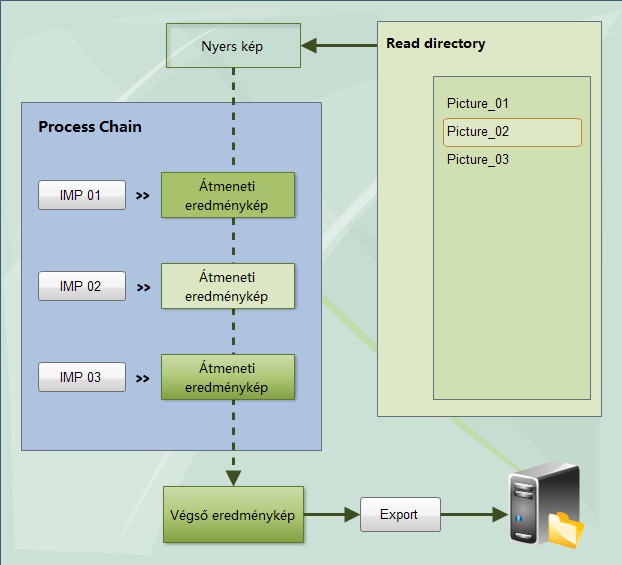
\includegraphics[width=0.8\textwidth]{read-dir-processing_IMP.jpg}
    \end{center}
	  \caption{A rendszer vázlatos működése}
	  \label{fig:bimg_usecase_brief}
\end{figure}


Az  \ref{fig:bimg_usecase_brief}. ábrán láthatjuk a rendszer vázlatos működését. Jelen példában egy könyvtárban található összes digitális képet kívánjuk feldolgozni. A beolvasás után a nyers képet átadjuk a feldolgozást végző logikának (ProcessChain), ahol jelen példában 3 darab elemi művelet történik (IMP01-03). A feldolgozás utolsó lépése után, a végső eredménykép (jelen esetben) exportálásra kerül, egy a bementi könyvtárral nem megegyező könyvtárba.

Fontos megjegyezni, hogy a feldolgozás pipelining \cite{book:pipelining_def} jelleget követ, tehát apró elemi lépések sorozata, amelyek kötött sorrendben végzik feladataikat. A műveletekből egy irányított gráf írható fel. Ahol a csúcspontok a műveleti egységek, az irányított élek pedig az adatok áramlása. (Ilyen műveleti módra jó példa különböző grafikus engineknél a fények számítása pl.: \cite{website:valve_shading_tree}. )

\section{Hasonló célú rendszerek}
Következő lépésként megvizsgáltam, hogy milyen hasonló célú szoftverek, illetve szoftvercsomagok találhatóak meg a piacon. Erre azért volt szükség, hogy pontosabb képet kapjak a jelenleg fellelhető megoldásokról, és munkám során az így szerzett pozitív és negatív tapasztalatokat eredményesen hasznosíthassam.

Különböző összehasonlítási szempontokat állítottam fel, melyek lentebb olvashatóak. Az vizsgálat során a személyes benyomáson túl, egyéni véleményeket is figyelembe vettem (pl.: kiadó cégnek vagy alapítványnak az ajánlása, vagy független publikáció, újságcikk).
\subsection{Összehasonlítási szempontok}

\subsubsection{Általános tulajdonságok}
\begin{itemize}
	\itemsep0em
	\item Platform: Milyen környezetben és operációs rendszeren használható? Milyen eszközökkel fejlesztették? \\Hordozhatósági szempontonból került be a listára.
	\item Licence: Milyen licenc alatt került publikálásra?\\Elsősorban pénzügyi és kód újrahasznosíthatósági jellemzők miatt érdekes.
	\item Cél csoport: A szoftver kinek az igényeinek a kielégítésére törekszik?\\Legtöbb esetben a célcsoport már alapvetően meghatározza, hogy a szoftverbe milyen funkcionalitásokat építünk be, illetve, hogy ezekhez milyen interfészt biztosítunk a jövőbeni felhasználóink részére.
	\item Támogató: Van hivatalos támogatása? (cég, alapítvány)\\Az esetek jelentős részében megfigyelhető, hogy egy szoftver, szoftvercsomag akkor válik igazán jól támogatottá, ha fejlesztői közösségen kívül egy nagyobb szervezet is gondozásába veszi.
	\item Felhasználói közösség: Fórum, levelező listák?\\Bármilyen előre nem látható hiba történhet: Ami elromolhat az el is romlik! A fenti csatornákon segítséget kérve nagy eséllyel kaphatunk választ kérdésünkre, és megoldást problémáinkra.
	\item Plugin rendszer: Plugin betöltésre van lehetőségünk? Saját plugin?\\A képfeldolgozás egy eléggé sokrétű szerteágazó lehetőségeket, funkcionalitásokat magában foglaló szakterület. Így az csak utópisztikus álom, hogy egyszer valaki implementálja az összes funkcionalitást és onnantól kezdve mindenki boldogan használja azokat az idő végezetéig\dots Ezért ha a program dinamikusan bővíthető (akár a felhasználó által készített bővítményekkel), jelentős előnyt jelent a többi monolitikus rendszerrel szemben.
	\item Kötegelt feldolgozási lehetőség: Feldolgozhatunk egyszerre nagy mennyiségű képet?
	\item Automatizálási lehetőségek: Automatizálhatjuk a feldolgozást?\\Ha lehetőségünk van a meglévő egyszerű feldolgozási lépéseket testreszabni, esetleg összekombinálni akkor az szintén egy jelentős előny lehet, más ilyen lehetőségekkel nem rendelkező szoftverekkel szemben.
	\item Fejlesztői eszközök: Rendelkezik hivatalos fejlesztői eszközökkel?
	\item Támogatott bemeneti formátumok köre
	\item Megjelenítési, vizualizációs lehetőségek listája, módjai\\Hasznos ha többféle interfészt biztosítunk az adott információ megjelenítéshez: más logikai kontextusban helyezve új megfigyeléseket is tehet a felhasználónk.

\end{itemize}


\subsubsection{Képfeldolgozási képességek}
\begin{itemize}
	\itemsep0em
	\item Képjavító eljárások, pl.: élesítés, kontrasztkiegyenlítés
	\item Geometriai műveletek, pl.: átméretezés, forgatás, tükrözés
	\item Analizálás, pl.: eltérések detektálása, alacsony szintű képleírók
	\item Szerkesztési műveletek, pl.: logikai, szöveg, alakzatok elhelyezése
	\item Színterek közötti konverzió, pl.: RGB $\rightarrow $ HSL, csatornák külön kezelése stb

\end{itemize}

\subsection{Választott szoftverek}
\begin{itemize}

    \item \emph{ImageJ}\cite{website:imagej}\\
    Képfeldolgozást és analizálást végző rendszer, amely a National Institutes of Health fejlesztése.
	A program első indulásakor látható, hogy itt egy professzionális orvostechnológiai eszközről van szó.
	Támogatottsága jelentős mind közösségi, mind bővíthetőségi szempontból. Eszközkészletének palettája széleskörű, külön kiemelném Z és T funkciókat.\cite{article:imagej_article}\\A Z funkciók segítségével pl.: MRI-vel készített sorozatos metszeti képeket kezelhetünk könnyedén, lehetőségeinket tovább növeli, hogy a térbeli szervezés mellett még időbeli struktúra felépítésére és kezelésére is lehetőséget ad a program (T funkciók).
    
    \item \emph{ImBatch}\cite{website:imbatch}\\
    Képfeldolgozást végző rendszer. Célcsoportja egyértelműen egy fél professzionális felhasználói szint. Tehát itt eleve nem is várunk professzionális analitikai funkciókat. Cserébe kapunk egy szép, letisztult, egyszerű grafikus felhasználói felületet, és egy pár használatot segítő kényelmi funkciót: pl.: Windows helyérzékeny menü integrációt.
    
    \item \emph{OriginLab - Image Processing}\cite{website:originlab}\\
	Az OriginLab szoftver csomag része, amely első sorban tudományos és ipari célközönséget szolgál ki. \cite{website:originlab_about} A korábban tárgyalt rendszerekkel ellentétben ez a szoftver fizetős (21 napos teszt verzió igényelhető). Ára hozza az iparban szokásos szoftver árakat \cite{website:originlab_usd}, amely személyes felhasználásra kissé borsos, azonban funkcionalitása kárpótolja a felhasználót. Rengeteg elemzési lehetőség mellett még OriginC-ben saját algoritmusainkat is megvalósíthatunk, a LabView támogatás már majdnem, hogy csak hab a tortán.\\
\end{itemize}
	

\subsection{Összefoglalás}
\subsubsection{Tapasztalatok}
A részletes összehasonlítás az \ref{table:diff_soft}. táblázatból olvasható ki a \pageref{table:diff_soft}. oldalon.\\

Az adatsorok elemzése közben, több fontos követelmény, fejlesztési irányvonal körvonalazódott:
\begin{itemize}
	\itemsep0em
	\item Hordozható legyen több platformra. Hiszen egy laboratóriumban több féle architektúra előfordul. (Ideális esetben tehát a szoftverünk legyen crossplatform.)
	\item Nyitott legyen a további fejlesztésekre. A felhasználónak adjuk meg a lehetőséget, hogy testre szabhassa a szoftverünket, vagy akár önmaga is fejlesztővé válhasson, így bővíthesse a pluginek körét, vagy javíthassa a fő programot.

	\item Szerepeljenek automatizálási lehetőségek. Írhassunk makrókat, vagy vizuális módon szerkeszthessünk algoritmusokat.
	\item A rendszert ajánlott az adott részterületen leggyakrabban előforduló, és legnépszerűbb ki- és  bemeneti adatformátumokra felkészíteni.
	\item Már gyárilag nagy mennyiségű képjavító, feldolgozó, szerkesztő, elemző és analizáló funkcionalitással érkezzen a szoftver.

\end{itemize}


\subsubsection{Célok}
Összegezve láthatjuk, hogy eléggé könnyen lehet már előkészített rendszereket választani a szoftverpiac palettájáról. Ilyenkor jogosan felmerül a kérdés, hogy ez a projekt miben ad többet, mint a jelenlegi lehetőségek? 
\begin{itemize}

\item Célom, hogy a programba új funkciók integrálása ne ütközzön problémákba, és az ilyen módon implementált funkcióknak a főprogramtól függetlenül is terjesztőknek kell lenniük. Ez természetesen maga után vonzza, hogy a plugin és főprogram közötti interfésznek kellően kompaktnak és univerzálisnak kell lennie, hogy több verzióváltás alatt is változatlan lehessen.

\item A sok kis méretű funkció egy idő után kezelhetetlenné válik, ezért legyen lehetőség kategorizálásra.

\item Legyen lehetőség átlátható szerkezetű grafikus felhasználói felület használatára. Erre kifejezetten alkalmas a blokkos kapcsolat alapú vizuális szerkesztő. Ez a módszer több különböző technológiai területen sikeresen vizsgázott pl.: Labview blokkdiagramjai \cite{website:ni_blocks}, vagy UDK4 BluePrint Editorja\cite{website:udk_blueprint} (amely az UDK3 Kismetjének egy tovább fejlesztett változata).
\end{itemize}


\begin{landscape}
\begin{table}[h]
\subsection{Hasonló célú rendszerek összehasonlítása táblázat}

\begin{tabular}{@{}rccc@{}}
\toprule
\multicolumn{1}{c}{\textbf{}} & \textbf{ImageJ} & \textbf{ImBatch} & \textbf{OriginLab} \\ \midrule
\textbf{Platform} & Multi (Java) & Win (C\#) & Win (C/C++) \\
\textbf{Licence} & Public Domain & Free  &  Commercial \\
\textbf{Cél csoport} & professzionális (orvosi) & félprofesszionális (általános) & professzionális (tudományos, ipari) \\
\textbf{Támogató} & National Institutes of Health & High Motion Software & OriginLab \\
\textbf{Felhasználói közösség} & \begin{tabular}[c]{@{}c@{}}wiki, leírások,\\ fejlesztői dokumtáció,\\ levlista, fórum\end{tabular} & \begin{tabular}[c]{@{}c@{}}gyik, leírások,\\ oktató videók\end{tabular} & \begin{tabular}[c]{@{}c@{}}gyik, wiki, leírások,\\ fejlesztői dokumentáció,\\ fórum\end{tabular} \\
\textbf{Plugin rendszer} & igen & igen & igen \\
\textbf{Kötegelt feldolgozás} & igen (Z-T funkciók) & igen (akár helyérzékeny menü) & igen \\
\textbf{Automatizálás} & makrók & részben & originC \\
\textbf{Fejlesztői eszközök} & igen & igen & igen \\
\textbf{Bemeneti formátumok} & széleskörű (orvosi irány) & széleskörű (általános irány) & széleskörű (ipari irány) \\
\textbf{Megjelenítés, GUI} & komplex & egyszerű letisztult & komplex \\
\textbf{Képjavító eljárások} & igen & igen & igen \\
\textbf{Geometriai műveletek} & igen & igen & igen \\
\textbf{Analizálás} & igen & nem & igen \\
\textbf{Szerkesztési műveletek} & igen & igen & igen \\
\textbf{Színterek közötti konverzió} & igen & igen & igen \\ \bottomrule
\end{tabular}
\caption{Hasonló célú rendszerek összehasonlítása}
\label{table:diff_soft}

\end{table} 
\end{landscape}


\section{Rendszertervek}
A következőkben röviden összefoglalom a szakdolgozat tárgyát képező szoftver terveinek elő-, és elkészítésének menetét. A korábbi fejezet végén vázolni kezdtem a programmal szembeni elvárásokat, javaslatokat, ez gyakorlatilag a követelményrendszer felírásának a kezdeti lépése volt. Természetesen a jelenlegi követelményrendszer kialakítását még megelőzte több beszélgetés, konzultáció is.\\
A megbeszélések során több logikailag összetartozó objektum, folyamat került felírásra. Ezek rendre nevet kaptak a kommunikáció hatékonyságának növelése érdekében. A legfontosabb elnevezéseket a \ref{table:szoszedet} táblázat prezentálja.

\begin{table}[h]
\subsection{Szószedet}
%\begin{tabular}{@{}rl@{}}
\begin{tabular}{p{3cm}|p{10cm}}

\toprule
\multicolumn{1}{c}{\textbf{Elnevezés}} & \multicolumn{1}{c}{\textbf{Definíció}} \\ \midrule
\textbf{BIMG} & A főprogramnak az elnevezése (képzése a Batch Image szavakból történt szóösszerántással). \\
\hline
\textbf{Modul} & BIMG-n belüli logikai egység. \\
\hline
\textbf{Plugin} & BIMG dinamikus kiterjesztése, az IMP Node-k lelőhelye \\
\hline
\textbf{IMP vagy Node} & Image Process Node, képfeldolgozási alapegységnek tekinthetjük, egy IMP általában egy jól körülhatárol művelet elvégzésére alkalmas. Három típusa van: adat (DataNode), indikátor (IndicatorNode), és feldolgozó (ProcessNode) \\
\hline
\textbf{Slot} & IMP Node be- és kimeneti interfészei. Egy slot egy paramétert párt kezel és tárol. \\
\hline
\textbf{Parameter vagy Paraméter} & Tetszőleges típusú adat. (pl.: szám, szöveg, kép) \\
\hline
\textbf{Slot Connection vagy kapcsolat} & Kettő darab azonos típusú paraméter tartalmazó slot között kapcsolat hozható létre. Ezt a kapcsolatot nevezzük Node Slot Connection-nek, vagy kapcsolatnak. Kapcsolat csak kimeneti és bemeneti slotok között jöhet létre. Az irány kötelezően: Ki-Be. \\
\hline
\textbf{ProcessChain} & Node-kat tartalmaz, és vezérli a feldolgozást. \\

\hline
\end{tabular}
\caption{Szószedet}
\label{table:szoszedet}
\end{table}
 A továbbiakban ezeket az elnevezéseket használom az adott objektumokra.




\subsection{Követelmény analízis}
A követelmény analízist a RUP (Rational Unified Process) metodika FURPS+ rendszerének útmutatása alapján végeztem. \\Célom az volt hogy a legtöbb tulajdonság és jellemző feltüntetésre kerüljön, amely szükséges, hogy a szoftver megoldja az adott problémát. \cite{website:soft_req_def} Ezek a követelmények jellemzőjüket tekintve lehetnek funkcionális követelmények, és nem funkcionális követelmények.

\subsubsection{Funkcionális követelmények}
Funkcionális követelményeknek tekintünk minden olyan követelményt, amely a fő termékünkbe valamilyen képességet biztosít. \cite{website:soft_func_req_ibm} Azaz ide tartozik minden felhasználói, cél feladat és aktivitás. Erre egy kitűnő eszköz a usecase, melyet legegyszerűbben a usecasediagramm segítségével tekinthetünk át.
\\
A \ref{fig:bimg_usecase_schema}. ábrán megfigyelhető a BIMG sematikus usecase diagramja\footnote{Megjegyzés: a vázlatos ábrázolás és a könnyebb szemléltetés miatt, a felhasználó csak a funkcionalitások csoportjaival és nem a külön-külön a funkcionalitásokkal került összekötésre.}.
\begin{figure}[h]
  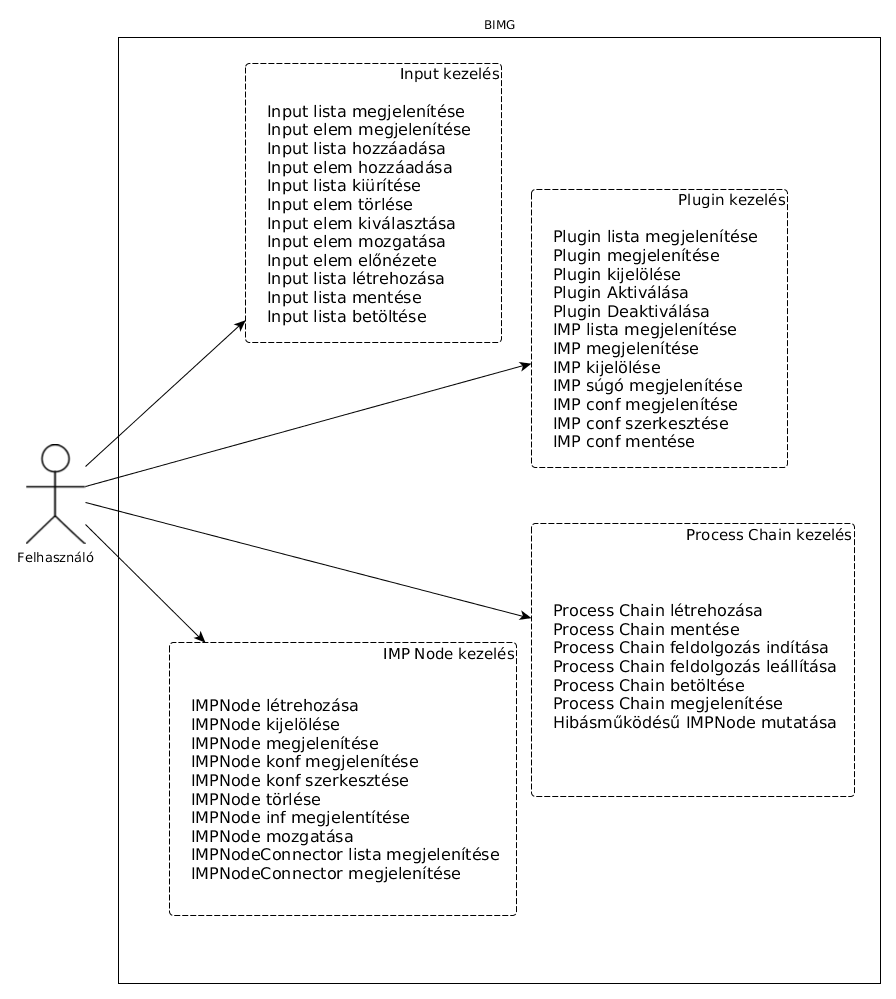
\includegraphics[width=\textwidth]{schematic_usecase.png}
  \caption{A BIMG sematikus usecase diagramja }
  \label{fig:bimg_usecase_schema}
\end{figure}



Az ábráról is egyértelműen leolvashatóak rendszert képző legfontosabb logikai egységek:
\begin{itemize}
	\itemsep0em
	\item Input kezelés: a funkcionalitásokból láthatjuk, hogy egy bemeneti elemekből azaz nyers képekből álló struktúrát tudunk managelni.
	\item Plugin kezelés: itt töltődnek be a feldolgozó egységek és az ezekhez tartozó esetleges, speciális adattagok is. Fontos megjegyezni, hogy szükség van az adattagok közötti konverziós lehetőségek definiálására is, hiszen így lesznek képesek a különböző fejlesztésű node-k egymással hatékonyan kommunikálni és együttműködni.
	\item Node kezelés: a pluginekből beolvasott node-k kezelése történik ezen a szinten.
	\item ProcessChain kezelés: Ezen a szinten találjuk meg azokat a funkciókat, amelyek a felhasználó számára lehetőséget adnak a feldolgozási folyamat definiálásra, szerkesztésére és tesztelésére.
	\item Feldolgozás: Ezen a szinten történik a feldolgozás összehangolása és az eredmények vizualizálása.
\end{itemize}
A teljes diagramm a \ref{fig:bimg_usecase_full}. ábrán tekinthető meg a. A kifejtett usecase a mellékletben csatolva olvasható: \emph{BIMG-usecase.pdf}



\subsubsection{Nem funkcionális követelmények}
A nem funkcionális követelmények halmazába tartozik minden, olyan követelmény, amely valamilyen korlátot, megszorítást vagy minőség irányú feltételt definiál. \cite{publication:soft_nonfunc_req} Természetesen ide a futásidejű követelményeken túl (mint pl.: megbízhatóság, teljesítmény, hibakezelés), ideértjük a fejlesztési követelményeket is (pl.: modularitás, bővíthetőség, kód újrafelhasználás stb). Először összegyűjtöttem a legfontosabb nem funkcionális követelményeket, majd ezeket osztályoztam, hogy az (F)URPS+ metodika melyik osztályába tartoznak. Ehhez jó kiindulási pont volt a témakiírás és a konzultációs beszélgetések.

\begin{table}[h]
%\begin{tabular}{@{}rl@{}}
\begin{tabular}{p{3cm}|p{10cm}}

\toprule
\multicolumn{1}{c}{\textbf{Típus}} & \multicolumn{1}{c}{\textbf{Követelmény}} \\ \midrule
\textbf{Modularitás és bővíthetőség} & A paraméterezhető képfeldolgozási algoritmusokat dinamikusan betölthető modulok biztosítsák a rendszer számára.\\
\hline
\textbf{Használhatóság} & A könnyen kezelhető grafikus felhasználói felületen legyen mód többlépcsős feldolgozásra. \\
\hline
\textbf{Támogatás} & Amennyiben a felhasználói felület használata nem teljesen triviális, készüljön hozzá kezelési leírás. \\
\hline
\textbf{Teljesítmény és megbízhatóság} & A rendszer legyen képes nagy mennyiségű bemenet feldolgozására. \\
\hline
\textbf{Megbízhatóság} & Egy esetleges hibás működésű modul ne okozzon rendszer szintű problémát. \\
\hline
\textbf{Implementáció} & A fejlesztés lehetőleg modern, ingyenes, nyílt-forrású  technológiákkal történjen. \\ 
\hline
\textbf{Interfész} & Több ki és bemeneti formátum támogatása. \\
\hline
\end{tabular}
\caption{A legfontosabb nem funkcionális követelmények}
\label{table:nonfunct_req_table}
\end{table}

\subsection{A feladat modellezése - Domain modell}
A követelmény analízist a megoldandó feladat részletes elemzése és modellezése követte. Erre az egyik legszélesebb körben használt eszköz a domain modell. Előnye, hogy kevés objektummal egyszerűen, és érthetően tudjuk ábrázolni a megoldani kívánt problémakört és feladatokat.\cite{book:usecase_book_brief}
\begin{center}
\begin{figure}[h]
  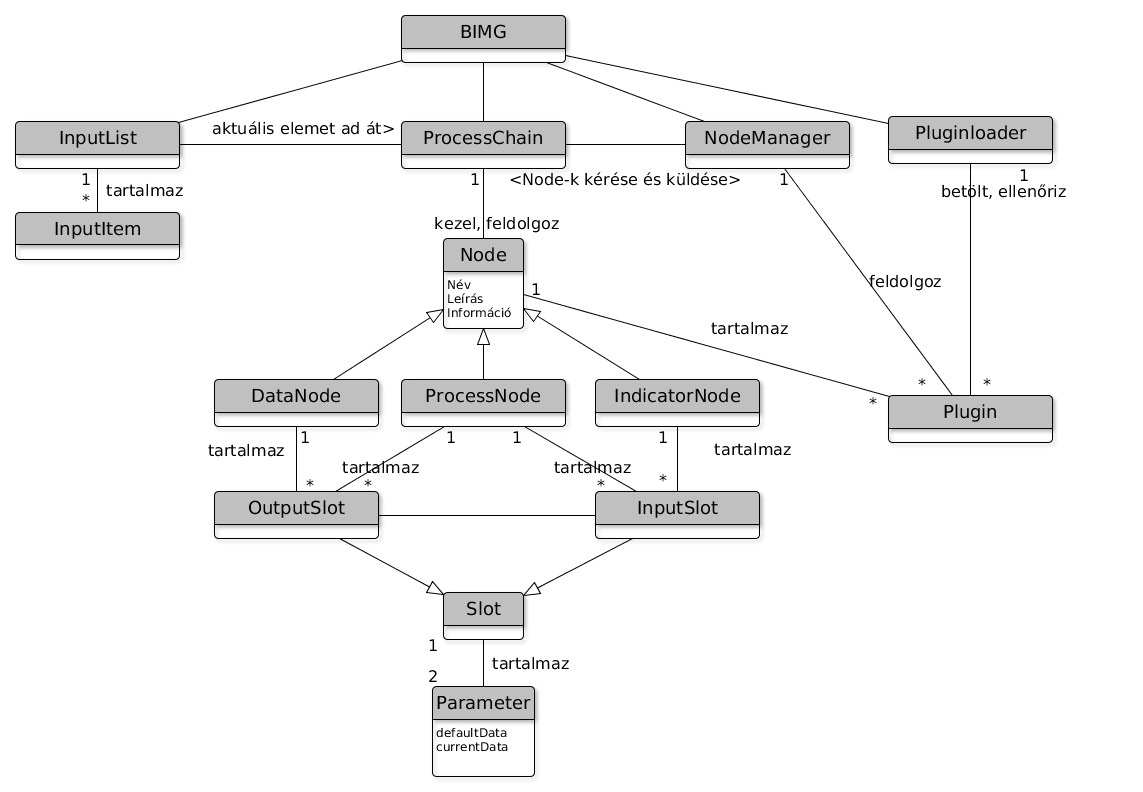
\includegraphics[width=1.1\textwidth]{domain_real_gray.png}
  \caption{A probléma ábrázolása domain modellen. }

  \label{fig:bimg_domain_minimal_img}
\end{figure}
\end{center}
A problémát bemutató domain modell a \ref{fig:bimg_domain_realworld_img}. ábrán látható. Itt szeretném megjegyezni, hogy ez a modell nem az egész rendszer ábrázolja. Itt csak alaprendszerek vázlatos bemutatására szorítkozom: Node-Slot-Parameter, ProcessChain, Input, Plugin, Node Management. A teljes modell a \ref{fig:bimg_domain_img}. ábrán az \pageref{fig:bimg_domain_img}. oldalon látható. A többi alrendszerről pedig a későbbiekben lesz szó, hiszen azok, már jelentős mértékben függenek a választott technológiáktól, és nem képzik szerves részét az alap logikának.

\subsubsection{Az alap rendszer - modell}
A BIMG alapját a Node-Slot-Parameter rendszer képezi. Paraméter lehet bármilyen tetszőleges adat (szám, szöveg, kép, vektor, mátrix stb).\\ Minden slotnak kötelezően két paraméterrel kell rendelkeznie, amíg az első az alapértelmezett értéket, addig a második az éppen aktuális értéket reprezentálja. A két érték típusa mindig azonos. Így látható, hogy a slotok csoportosíthatóak  tárolt adattípus szempontjából. Azonban ezen túlmenően működési irány alapján is rendszerezhetőek. Az irány azt reprezentálja, hogy az adott slot az őt tartalmazó node-ban milyen irányú kommunikációt képes végezni.
\begin{itemize}
	\itemsep0em
	\item InputSlot: Bemeneti kommunikációt végez, így bemeneti adatot reprezentál a node szempontjából. Alapértelmezetten blokkolja a node végrehajtását.
	\item OutputSlot: A node szempontjából kimeneti adatot reprezentál, hiszen kimeneti kommunikációt végez. A node végrehajtását nem blokkolja.
\end{itemize}
Összegezve beszélhetünk akár pl.: bemeneti számot, kimeneti képet stb kezelő slotokról. Egy slot csak egy nodehoz tartozhat, de egy node több slotot is foglalhat magában.
Három fajta node létezik a rendszerben:
\begin{itemize}
	\itemsep0em
	\item DataNode: Csak Output slottal rendelkezik, tehát a teljes feldolgozás szempontjából egyértelműen csak bemeneti adatforrásnak tekinthető. Mivel nincsen bemeneti slotja azonnal végrehajtható. Alapvető funkciója: adatot juttat be a ProcessChainbe.
	\item IndicatorNode: csak Input slottal rendelkezik, tehát a teljes feldolgozás szempontjából csak kimeneti adatforrásként kezelhető. Alapvető funkciója: adatot juttat ki a ProcessChainból.
	\item ProcessNode: Input- és OutputSlotokkal is rendelkezik. Az egyetlen node típus, amely igazi feldolgozási logikával rendelkezik (tehát nem csak megjelenít, vagy vissza adértékeket, hanem azokkal tényleges műveletet is végez). Végrehajtása az InputSlotok miatt alap esetben blokkolt. Alapvető funkciója: feldolgozás.

\end{itemize}
A nodek között slotok segítségével kapcsolat építhető fel. A node-k a végrehajtását a ProcessChain ütemezi és irányítja. Az éppen feldolgozásra szánt kép az InputListről érkezik, amelyet a ProcessChain átvesz. Az InputListben több elem is található, mindegyik egy nyers eredményképet reprezentál.\\
A nodek pluginekben kerülnek a rendszerbe. A plugineket a pluginmanager tölti be induláskor automatikusan, majd validálás után a plugin nyers tartalmát tovább adja a NodeManagernek. A NodeManger az átvett nyers plugin tartalmat, amely, különböző BIMG által használt objektumok listái, feldolgozza, és regisztrálja az adott node típust. Amennyiben a felhasználó a ProcessChaint egy új noddal szeretné bővíteni, a ProcessChain kérést intéz a NodeManagerhez, ami ha a kért node típus érvényes és regisztrált elkészít egy példányt, és visszaadja a ProcessChain számára.

\begin{landscape}
\begin{figure}[h]
  \subsection{Domain modell}
  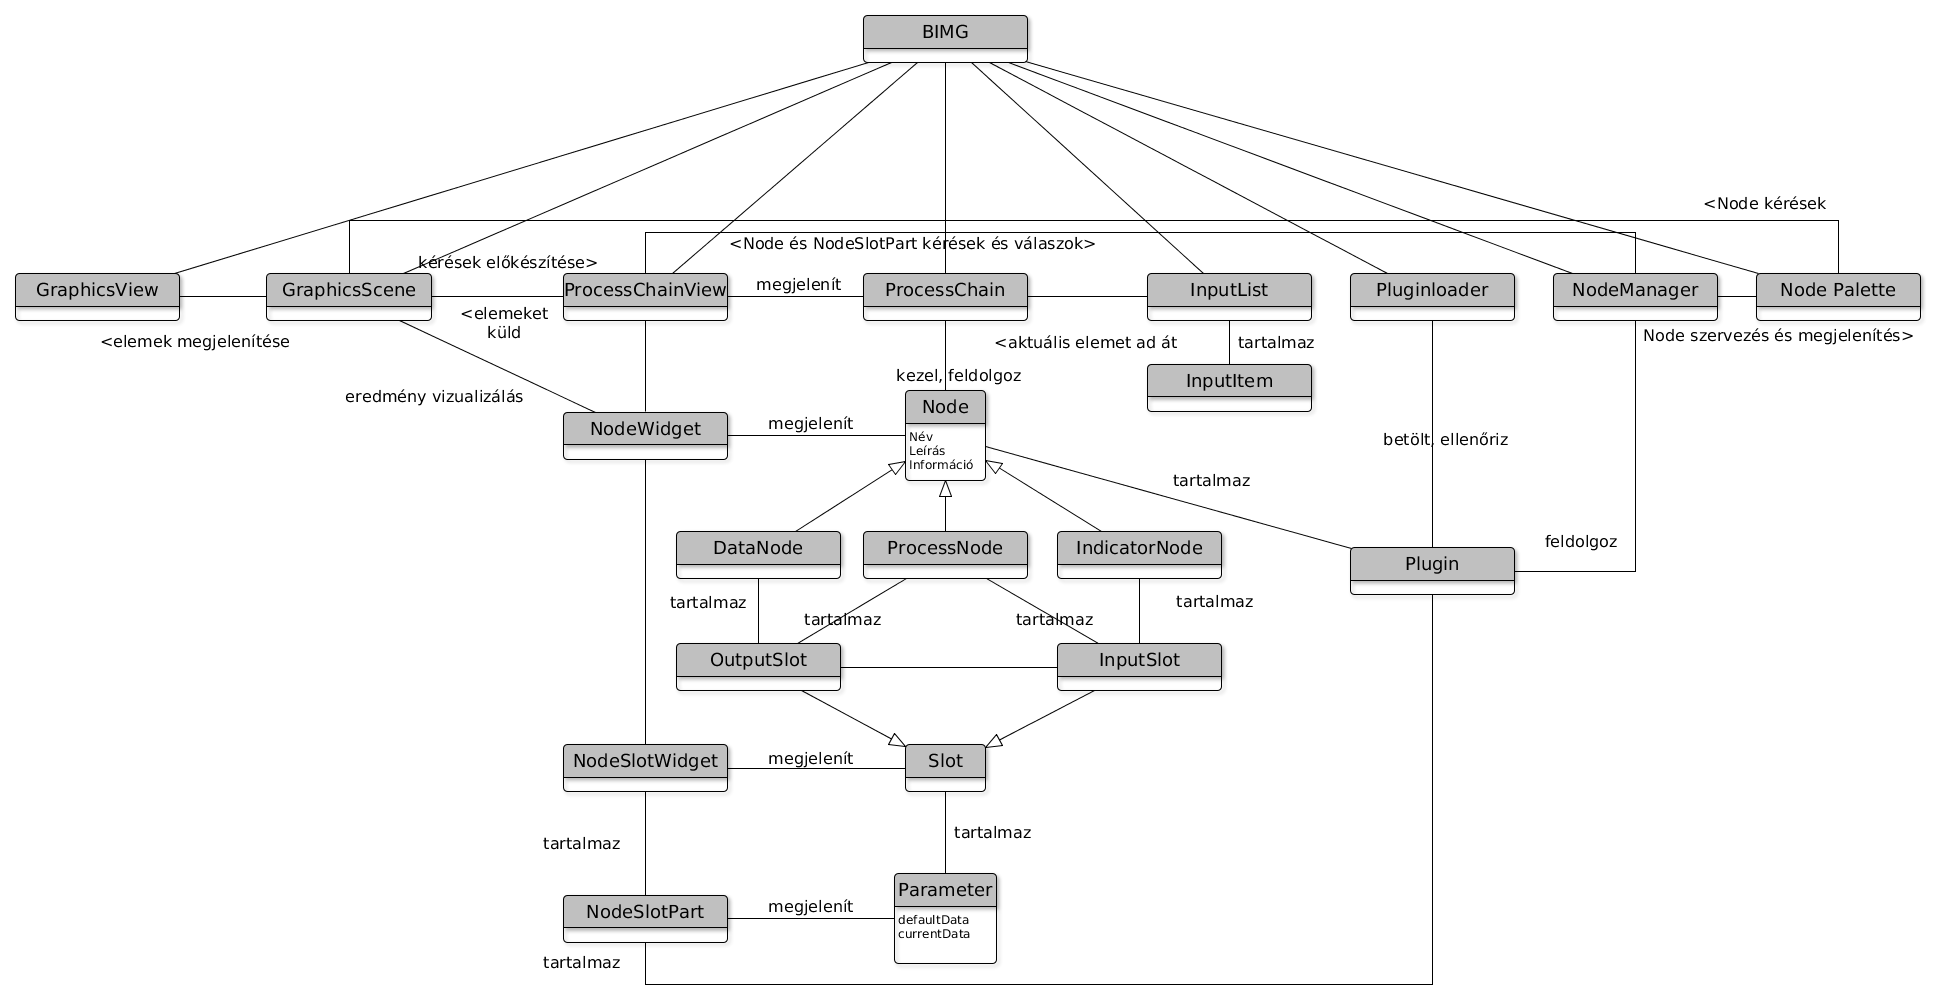
\includegraphics[width=26cm,height=30cm,keepaspectratio]{domain_gray.png}
  \caption{A domain modell állapota az utolsó fejlesztési iteráció végén }

  \label{fig:bimg_domain_img}
\end{figure}
\end{landscape}

\subsection{Választott technológiák}
A feladat modellezése után döntést kellett hoznom, hogy milyen technológiákkal kívánom megvalósítani a tervezett rendszert. Több tényező is befolyásolta a döntésemet. Ezekből két nagy csoportot írtam fel: a feladatból illetve szubjektív nézőpontból kiemelt fontosságú szempontok. A feladatból, és követelményrendszerből adódóakat a korábbi fejezetekben már részleteztem, ezért a következőkben csak a szubjektív pontokat vázolnám fel.
\begin{itemize}
	\itemsep0em
	\item Egyszerű és gyors, minőségi fejlesztés
	\item Könnyű dokumentálhatóság
	\item Legyen korábbi munkáimból rutinom az adott technológiák alkalmazásában
	\item Képfeldolgozási függvénykönyvtárakkal legyenek jól ellátottak a kiválasztott technológiák (nem szeretném újra feltalálni a kereket)
\end{itemize}
A program alap szerkezete Qt-val, a képfeldolgozásért felelős komponensek OpenCV-vel történő implementálása mellett döntöttem. A verziókövetést Git-el végeztem, a dokumentáció és dolgozat elkészítéséhez pedig Latex-et, Gummi-t, Doxygen-t, és Yed-et használtam.
\subsubsection{Qt}
Egyike a legmeghatározóbb\cite{website:qt_1_million} multiplatform c++-ra épülő alkalmazás keretrendszereknek. \cite{website:qt_about} Korábban már több másik projektben is sikeresen dolgoztam vele. A részletes dokumentáció és aktív felhasználói/fejlesztői bázis sokat segített a fejlesztésben. \cite{website:qt_dochome} \cite{website:qt_docforum}\cite{website:qt_docmaillist} Licencelése kedvező, elérhető OpenSource és Enterprise verziója is. Olyan nagy cégek is használják mint a BlackBerry, Michelin vagy a Panasonics.\cite{website:qt_in_use} \\ A fejlesztés korai fázisa az 5.1es verzióval történt, azonban az új 5.2es verzió jelentős újításokat hozott (főként a metatype rendszer szempontjából), ezért átálltam az 5.2.1-es verzióra.


\subsubsection{OpenCV}	
Open Source Computer Vision Library, nyílt-forrású képfeldolgozást, és gépi tanulást megvalósító függvénykönyvtár.\cite{website:opencv_about} Natív c++-ban implementált, és erősen támaszkodik azt stl tárolókra. Sajnos gyárilag csak c/c++ és phyton-al tud hatékonyan együttműködni. Szerencsére egy vékony wrapper elkészítésével könnyen összekapcsolható Qt-val is. Funkcionalitásával széleskörű feladatok megoldására kiválóan alkalmas, technológiai lehetőségek arzenálját vonultatja fel pl.: Cuda, OpenCl. Multiplatform, még okos telefonra is elérhető a portja (Android 2010, iOS 2012). Dokumentációja is megfelelő. Jelen programban a 2.4.8-as verzióval dolgoztam.


\section{Architekturális tervek és megvalósítási folyamatok}
A modellre építve a választott technológiák segítségével az első iterációban kidolgoztam a Node-Slot-Parameter alrendszert.
\subsection{Az alaprendszer - architektúra}
\subsubsection{Parameters}
Az első tervek alapján elkészült proof of concept templates slotokra épült, ahol a template paraméterként átadott objektum volt a slotnak a paramétere. Azonban sajnos hamar be kellett látnom, hogy ez a templates implementáció nem rendelkezik elég flexibilitással ahhoz, hogy hatékonyan teljesítse a feladatokat. A legnagyobb problémát az jelentette, hogy ha egyedi plugineket és nodekat készítünk akkor a rendszernek kell tudnia kezelni az esetleges új adattípusokat is. Az adattípusok kezelése alatt, nem csak az adott típusú slotok létrehozása, és managelése értendő, hanem a típusok közötti megfeleltetések, konverziók is. Tehát programnak valós időben kell ezeket az adattípusokat összegyűjteni, tárolni és rendszerezni.

Erre tökéletesen alkalmas a Qt-nek a metatype rendszere. Bármilyen tetszőleges osztályt metatípusként deklarálhatunk, így lehetőségünk van az adott objektumokat QVariantban eltárolni. \cite{website:qt_metatype_1} Mivel a metatípus azonosítók kiosztása, és feloldása valós időben történik, így megoldható a pluginekben található osztály definíciók a főprogramban történő használata.\\
A QVariant alapvető adattípusok számára biztosít konverziós lehetőséget. Az 5.2-es verziótól már arra is van lehetőségünk, hogy mi definiáljunk különböző metatípusok közötti konverziós műveleteket. \\ Az alábbi lehetőségeket összegezve egyértelmű volt a döntés, hogy a slot paraméterek a qt metatype rendszerre épülve kerülnek megvalósításra. (Az adattípusok betöltését és konverziók regisztrálását a pluginek működéséről szóló részben fejtem ki.)

\subsubsection{Slots}
A korábban említett templates architektúra elhagyása lehetővé tette, hogy a nodek slotjai is QObject alapokra épüljenek. Tehát a kommunikációjuk és így az adat továbbítás a nodek között a qt Signal/Slot mechanizmusára épülhessen.
\begin{center}
\begin{figure}[h]
  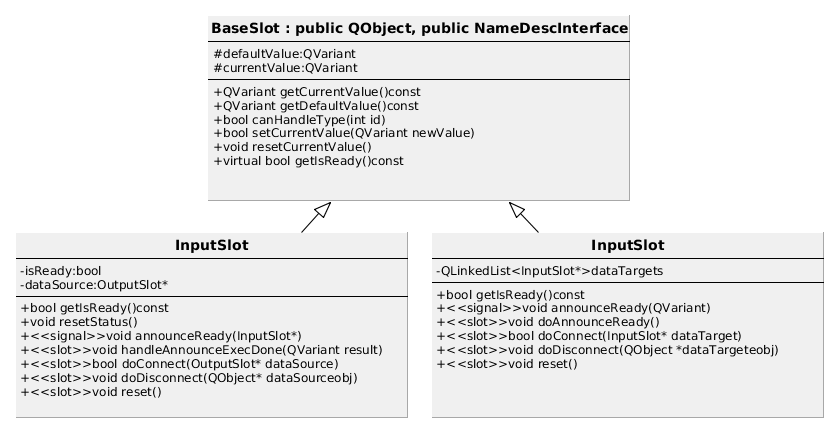
\includegraphics[width=1.1\textwidth]{slot_diag.png}
  \caption{A node slotok osztálydiagramja }

  \label{fig:bimg_slot_diag}
\end{figure}
\end{center}
A \ref{fig:bimg_slot_diag}. ábrán látható a slotok jelenlegi osztálydiagramja. A funkcionalitások szervezésekor (hogy mi kerüljön a BaseSlot osztályba és mi a gyermek slot osztályokba), a logika az volt, hogy a BaseSlot gyakorlatilag csak és kizárólag az aktuális, és az alapértelmezett paraméterek kezelését valósítsa meg, míg az input-, és outputslot pedig a paraméterek fölé biztosít egy réteget ami kezeli a slot kapcsolódásokat, és állapotokat. Ennek a döntésnek az oka annyi, hogy két fő szabályt osztály architekturális szinten kívántam megkötni:
\begin{itemize}
	\itemsep0em
	\item Egy input slothoz csak egy output slot kapcsolódhat.
	\item Egy output slot több input slotba is szolgáltathat adatot.
\end{itemize}
Tehát nem a doConnect() és a doDisconnect() függvények működése határozza meg a kapcsolódási mechanizmust, hanem az architektúre, hogy adott slot típus ne is tudjon más számú, és típusú kapcsolatot létesíteni. Tény, hogy ez eléggé erős megkötés, de a feldolgozás és nodek kiterjesztési sorrendje nagyon erőteljesen támaszkodik erre a két szabályra, így vált indokolttá ennek a döntésnek a meghozatala.

A kapcsolat mindig az inputslot irányából jön létre. Tehát amikor az outputslotnál kezdeményezzük a kapcsolat létrehozását az átadja a működést az cél inputslotnak. Ennek egyik oka a fent említett megszorítások: azaz inputslot felől szigorúbb a kapcsolat létrehozása, a másik oka, hogy így a kapcsolatot kezelő kódot csak egy helyen kell karbantartani és a későbbi esetleges fejlesztések nem okozhatnak inkonzisztens kapcsolódási állapotot.

A slotok közötti adatáramlás iránya outputslot - inputslot irányú. Az adatok átadása az outputslot által emitált announceReady(QVariant) signállal kezdődik, és az inputslot handleAnnounceExecDone(QVariant) függvényének meghívásával zárul. A két slot közötti kapcsolat a Qt signal-slot mechanikájával történik. Ez a működés megfigyelhető a \ref{fig:bimg_dataflow}. ábrán.

\subsubsection{Nodes}
Már a slotok osztálydiagramján is látható, hogy az alaposztály egy NameDescInterface osztálynak is a gyermekosztálya. Ez a kis interfész jellegű osztály általános adattagokat (és getter és setter függvényeket) biztosít bármely gyermek osztályának. Itt jellemzően a felhasználó munkáját könnyítő információk kerülnek tárolásra: az objektum olvasható neve, rövid leírása, és súgó szöveg.

\begin{center}
\begin{figure}[h]
  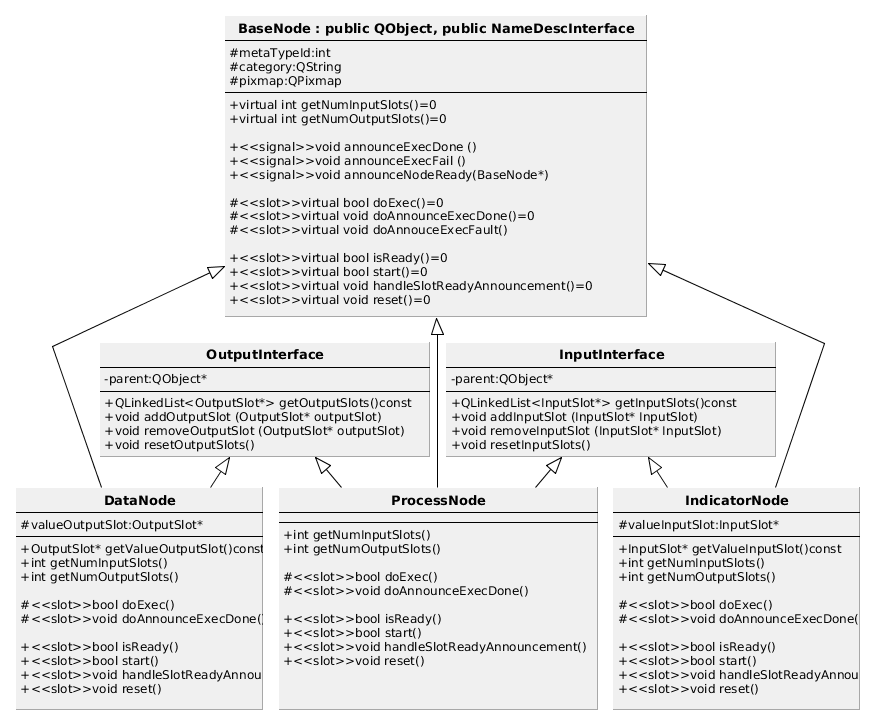
\includegraphics[width=1.1\textwidth]{node_class_diag.png}
  \caption{A node slotok osztálydiagramja }

  \label{fig:bimg_slot_diag}
\end{figure}
\end{center}

Bár az osztály diagramon nem látható egyértelműen, de a slotok BaseNode szinten tárolódnak. Mivel minden slot és node kötelezően QObject ezért kiválóan használhatóak a gyermek szülő funkciók. Ezek QObject szinten vannak implementálva. Használatuk jelentős előnyökkel jár pl.: a node átveszi a slot feletti irányítást: tehát amikor megszűnik a node automatikusan felszabadításra kerül az összes slot. A slot felszabadításakor emitálásra kerül egy destroyed(QObject*) signal, amely az adott slot doDisconnect(QObject*) slotjával van összekötve. Ezzel a struktúrával elértem, hogy egy node törlésekor a gyermek slotjainak az összes kapcsolata automatikusan felbontásra kerüljön. Ennek előnye, hogy nem maradhatnak érvénytelen kapcsolatok a rendszerben, amelyek már nem létező slotra mutatnak.

 A BaseNode osztály a slotok tárolásán és alacsony szintű kezelésén túl, definiál egy sor virtuális függvényt, melyekkel a magasabb szintű node kezelő és feldolgozó mechanizmusok (ProcessChain) számára biztosít interfészt. Az alapvető működésük, és a slotokkal történő interakciójuk megfigyelhető a \ref{fig:bimg_dataflow}. ábrán. Ezek közül a legfontosabb függvények működése:
\begin{itemize}
	\itemsep0em
	\item start(): Ez minden node belépési pontja a ProcessChain ezt a függvényt hívja meg végrehajtáskor, ha a node készen áll a végrehajtásra akkor lefut a benne található logika. A futás eredményét (sikeres vagy sikertelen) visszatérési értéke és az emitált signalok mutatják.
	\item reset(): Alapállapotba állítja vissza a nodet. Erre akkor van szükség amikor a ProcessChain egy új bemeneti adatot szeretne feldolgozni. Ilyenkor a node és az összes slotja felveszi az alapértelmezett állapotot.
	\item isReady(): Ellenőrzi a node inputslotjainak az állapotát, ha mindegyik slot készen áll a végrehajtásra (tehát már mindegyik input slot kapott bemeneti adatot), akkor igaz értéket ad vissza: tehát a node végrehajtható.
	\item handleSlotReadyAnnouncement(): Amikor bármelyik input slot ready állapotba vált akkor, ellenőrzi a teljes node állapotát (isReady()) ha végrehajtásra kész, akkor meghívja announceNodeReady(BaseNode*) függvényt
	\item announceNodeReady(BaseNode*): Jelzi a ProcessChain számára ha végrehajtásra kész állapotba került a node.
	\item doAnnounceExecDone() és doAnnouceExecFault(): a node végrehajtásának eredményét jelentik be.
	
	\item doExec(): Itt található a node feldolgozó logikája. Amennyiben valaki új nodet fejleszt ezt a függvényt kell felül definiálnia. 
\end{itemize}
Mivel a BaseNode osztály tervezésekor az volt a cél, hogy slot típustól függetlenül működjön ezért két segéd osztályt kellett definiálni. Ezek az OutputInterface és az InputInterface. Feladatuk egyszerű: egy szülőként kapott QObject-ből visszaadják az összes számukra kezelhető slot típust. Továbbá interfészt biztosítanak, hogy új slotokat adjunk a nodehoz és a régieket eltávolítsuk. Ha az adott interface osztályból örököltetünk akkor megkapjuk a lehetőséget, hogy az adott slot típusokkal dolgozzunk. Amennyiben a későbbiekben egy másik típusú slotot szeretnék elhelyezni a rendszerben pl.: ami csak konfigurációs segéd adatokat biztosít a node számára, akkor értelemszerűen készíteni kell egy interface osztályt, amiből ha örököltetünk már is rendelkezésre állnak az új típusú slotok.\\
Az osztálydiagramon látható örököltetésekből egyértelműen kiderül, hogy melyik node típus milyen slotokkal képes dolgozni. A DataNode csak outputot, az IndicatorNode csak inputot, a ProcessNode pedig mind a kettőt képes használni. A módszer előnye, hogy így kis apró szerepkörökből hamar össze lehet állítani a node működési területét, majd a BaseNode virtuális függvényei kifejtésével meghatározható a pontos működés.

\begin{landscape}
\subsubsection{Node-Slot adatáramlás}
Lenti ábrán megfigyelhető a nodek végrehajtási mechanizmusa során keletkezett, információk tovaterjedése a kapcsolódott nodekkal, továbbá a legalapvetőbb ProcessChain és node interakciók. (Működésükről bővebben a Nodes, és Slots alfejezetkben lehet olvasni.)
\begin{center}
\begin{figure}[h]
  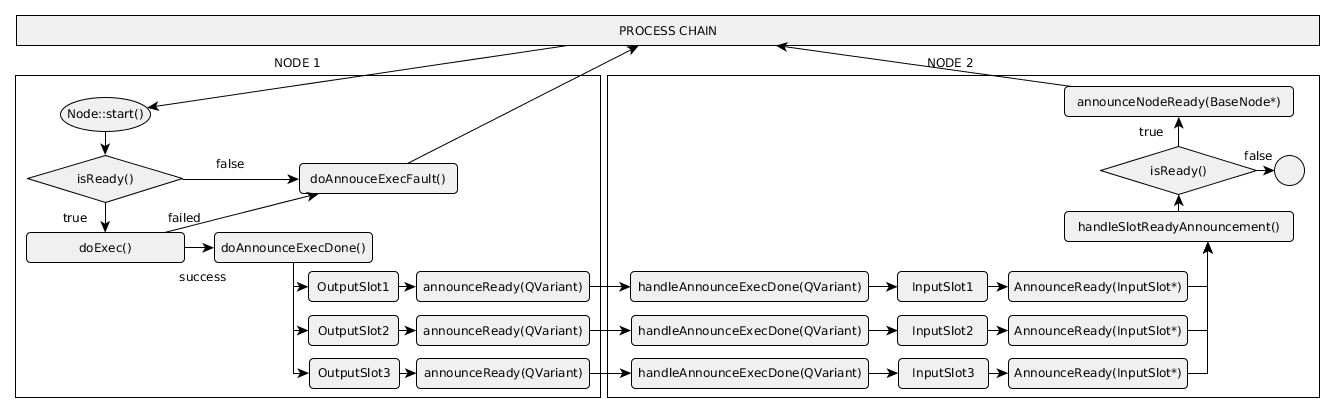
\includegraphics[width=23cm,height=30cm,keepaspectratio]{node-data.png}
  \caption{A Node-Slot adatáramlás }

  \label{fig:bimg_dataflow}
\end{figure}
\end{center}
\end{landscape}

\subsubsection{ProcessChain}
A korábbi pontokból látható, hogy a Node-Slot-Parameter alrendszerrel gyakorlatilag tetszőleges feldolgozási sor összeállítása lehetséges. Ez a feldolgozási sor tekinthető egy irányított gráfnak. Így az alábbi megfeleltetések jönnek létre:
\begin{itemize}
	\itemsep0em
	\item csúcsok: a feldolgozási sor nodejai,
	\item élek: nodek slotjai közötti kapcsolatok,
	\item élek iránya: a slotok kapcsolati irányának felel meg. (Outputslotból mutat inputslot felé.)
\end{itemize}
Az alábbi logika mentén tovább haladva a feldolgozási sort, tehát ahogy a nodeknak az egymás után történő sorrendhelyes végrehajtását tekinthetjük a gráf egy bejárásnak.\\
A gráf bejárására lehetőségünk van egy állapotgépet felírni. Az állapotgép jellemzői:
\begin{itemize}
	\itemsep0em
	\item Három darab memória területe van. L\textsubscript{0}, L\textsubscript{1} és L\textsubscript{2} 			\begin{itemize}
			\itemsep0em
			\item A memória területek között a nodekat átmozgatjuk, tehát nem másoljuk: így egy node mindig csak egy területen szerepelhet
			\item L\textsubscript{0} induláskor minden node itt található
			\item L\textsubscript{1}-ben tárolunk minden ready állapotú nodet (amelyek készen állnak a végrehajtásra)
			\item L\textsubscript{2}-ba kerülnek a már kiterjesztett nodek (itt jelenik meg a kiterjesztési sor)
		\end{itemize}
		
	\item Az állapotgép minden állapotában vagy egy művelet történik, a művelet eredménye lehet sikeres (1), és sikertelen (0), egy állapotból továbbléphetünk annak eredményétől függetlenül is. Tehát az abc: \{0,1,e\}
	\item Az állapotgép három esetben állhat meg:
			\begin{itemize}
			\itemsep0em
			\item Az összes node kiterjesztése sikeres volt: ez esetben a művelet egyértelműen sikeres volt.
			\item Nincsen további kiterjesztésre kész node. Ez esetben ha az L\textsubscript{0}-án nem maradt egy darab IndicatorNode sem, akkor a feldolgozást sikeres. (Hiszen előfordulhatnak izolált csúcsok a gráfban.) Azonban ha található a még nem kiterjesztett nodek között (L\textsubscript{0}) indicator node a feldolgozás sikertelen volt.
			\item Ha valamelyik node kiterjesztése sikertelen volt. (A kiterjesztés közben hiba lépett fel. Ezt többnyire a node nem megfelelően elkészített doExec() metódusában bekövetkezett hibát jelent.)

		\end{itemize}

\end{itemize}
\begin{center}\lstset { %
    language=C++,
    backgroundcolor=\color{black!5}, % set backgroundcolor
    basicstyle=\footnotesize,% basic font setting
}
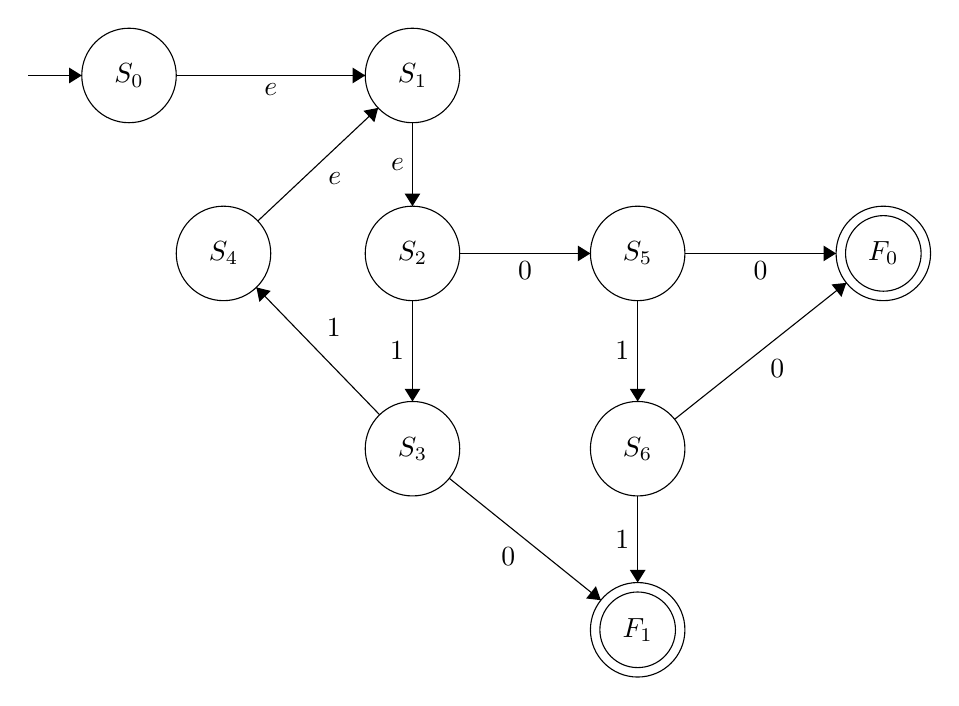
\begin{tikzpicture}[scale=0.2]
\tikzstyle{every node}+=[inner sep=0pt]
\draw [black] (5.5,-13.5) circle (3);
\draw (5.5,-13.5) node {$S_0$};
\draw [black] (23.5,-13.5) circle (3);
\draw (23.5,-13.5) node {$S_1$};
\draw [black] (23.5,-24.8) circle (3);
\draw (23.5,-24.8) node {$S_2$};
\draw [black] (37.8,-48.7) circle (3);
\draw (37.8,-48.7) node {$F_1$};
\draw [black] (37.8,-48.7) circle (2.4);
\draw [black] (53.4,-24.8) circle (3);
\draw (53.4,-24.8) node {$F_0$};
\draw [black] (53.4,-24.8) circle (2.4);
\draw [black] (23.5,-37.2) circle (3);
\draw (23.5,-37.2) node {$S_3$};
\draw [black] (37.8,-24.8) circle (3);
\draw (37.8,-24.8) node {$S_5$};
\draw [black] (37.8,-37.2) circle (3);
\draw (37.8,-37.2) node {$S_6$};
\draw [black] (11.5,-24.8) circle (3);
\draw (11.5,-24.8) node {$S_4$};
\draw [black] (-0.9,-13.5) -- (2.5,-13.5);
\fill [black] (2.5,-13.5) -- (1.7,-13) -- (1.7,-14);
\draw [black] (8.5,-13.5) -- (20.5,-13.5);
\fill [black] (20.5,-13.5) -- (19.7,-13) -- (19.7,-14);
\draw (14.5,-14) node [below] {$e$};
\draw [black] (23.5,-16.5) -- (23.5,-21.8);
\fill [black] (23.5,-21.8) -- (24,-21) -- (23,-21);
\draw (23,-19.15) node [left] {$e$};
\draw [black] (23.5,-27.8) -- (23.5,-34.2);
\fill [black] (23.5,-34.2) -- (24,-33.4) -- (23,-33.4);
\draw (23,-31) node [left] {$1$};
\draw [black] (25.84,-39.08) -- (35.46,-46.82);
\fill [black] (35.46,-46.82) -- (35.15,-45.93) -- (34.53,-46.71);
\draw (29.59,-43.44) node [below] {$0$};
\draw [black] (26.5,-24.8) -- (34.8,-24.8);
\fill [black] (34.8,-24.8) -- (34,-24.3) -- (34,-25.3);
\draw (30.65,-25.3) node [below] {$0$};
\draw [black] (40.8,-24.8) -- (50.4,-24.8);
\fill [black] (50.4,-24.8) -- (49.6,-24.3) -- (49.6,-25.3);
\draw (45.6,-25.3) node [below] {$0$};
\draw [black] (37.8,-27.8) -- (37.8,-34.2);
\fill [black] (37.8,-34.2) -- (38.3,-33.4) -- (37.3,-33.4);
\draw (37.3,-31) node [left] {$1$};
\draw [black] (40.15,-35.33) -- (51.05,-26.67);
\fill [black] (51.05,-26.67) -- (50.11,-26.77) -- (50.74,-27.56);
\draw (46.66,-31.49) node [below] {$0$};
\draw [black] (37.8,-40.2) -- (37.8,-45.7);
\fill [black] (37.8,-45.7) -- (38.3,-44.9) -- (37.3,-44.9);
\draw (37.3,-42.95) node [left] {$1$};
\draw [black] (21.41,-35.04) -- (13.59,-26.96);
\fill [black] (13.59,-26.96) -- (13.78,-27.88) -- (14.5,-27.18);
\draw (18.03,-29.53) node [right] {$1$};
\draw [black] (13.68,-22.74) -- (21.32,-15.56);
\fill [black] (21.32,-15.56) -- (20.39,-15.74) -- (21.08,-16.47);
\draw (18.57,-19.63) node [below] {$e$};
\end{tikzpicture}
\end{center}

\begin{table}[h]
%\begin{tabular}{@{}rl@{}}
\begin{tabular}{p{1cm}|p{12cm}}

\toprule
\multicolumn{1}{c|}{\textbf{Állapot}} & \multicolumn{1}{|c}{\textbf{Művelet}} \\ \midrule
\multicolumn{1}{c|}{\textbf{S\textsubscript{0}}}  & Kezdő állapot. \\
\hline
\multicolumn{1}{c|}{\textbf{S\textsubscript{1}}}  &  L\textsubscript{0}-án található összes ready állapotú átmásolásra kerül L\textsubscript{1}-re.\\
\hline
\multicolumn{1}{c|}{\textbf{S\textsubscript{2}}}  & Található elem L\textsubscript{1}-en? \\
\hline
\multicolumn{1}{c|}{\textbf{S\textsubscript{3}}}  & L\textsubscript{1} első eleme kiterjesztésre kerül. Sikeres volt?  \\
\hline
\multicolumn{1}{c|}{\textbf{S\textsubscript{4}}}  & A sikeresen kiterjesztett eleme L\textsubscript{1}-ről átmozgatásra kerül L\textsubscript{2}-re.  \\
\hline
\multicolumn{1}{c|}{\textbf{S\textsubscript{5}}}  & Található node L\textsubscript{0}-án? \\
\hline
\multicolumn{1}{c|}{\textbf{S\textsubscript{6}}} & Az L\textsubscript{0}-ás nodek között található IndicatorNode? \\
\hline
\multicolumn{1}{c|}{\textbf{F\textsubscript{0}}} &  A feldolgozás véget ért! Eredmény: SIKERES FELDOLGOZÁS!\\
\hline
\multicolumn{1}{c|}{\textbf{F\textsubscript{1}}} & A feldolgozás véget ért! Eredmény: SIKERTELEN FELDOLGOZÁS! \\
\hline
\end{tabular}
\caption{Az állapotgép állapotainak értelmezése }
\label{table:nonfunct_req_table}
\end{table}

Látható, hogy mennyire előnyös ez az állapotgépes feldolgozás, hiszen nem kell a gráfban kört keresni illetve egyéb más módon elemezni azt. Adott pár jól definiált művelet és szabály ami alapján egyértelműen végrehajtható a felhasználó által felépített feldolgozási sor. Az adatok áramlása és a nodek ready állapotba kerülése pedig alacsonyabb szinten teljes mértékben rendezésre kerül és a nodek elfedik azt a ProcessChain elől.

A korábbiakban bemutattam, hogy egy bemeneti elemre, hogyan működik a feldolgozás. Természetesen van lehetőség több elem egymás utáni feldolgozására is. Ennek feltétele, hogy miután egy adott bemeneti elem sikeresen feldolgozásra került exportáljuk az eredményt, majd alaphelyzetbe állítsuk a ProcessChaint és a benne található nodekat. A be-, és kimeneti adatokat az InputList biztosítja a ProcessChain számára. (Amelynek beállítása a populateNodesWithImage() függvényben történik.)\\
Megjegyzés: ha valamelyik bemeneti elem feldolgozása sikertelen volt akkor a ProcessChain ugyanúgy alapállapotba kerül vissza (a hibaüzenetek nyugtázást követően).

Az alábbi osztálydiagramon látható a ProcessChain legfontosabb adatagjai és függvényei.
\begin{center}
\begin{figure}[h]
  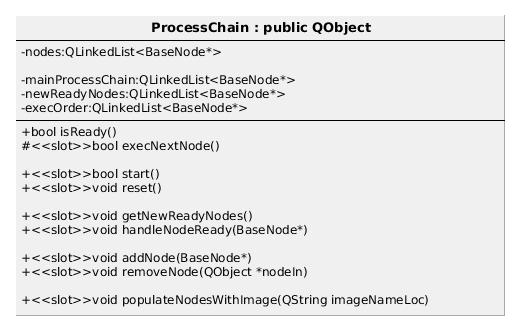
\includegraphics[width=1.0\textwidth]{process_chain_diag.png}
  \caption{ProcessChain osztálydiagramja }

  \label{fig:bimg_processchain_diag}
\end{figure}
\end{center}
Megfigyelhető a nodek általános tárolója (nodes), és L\textsubscript{0} (mainProcessChain), L\textsubscript{1} (newReadyNodes) és L\textsubscript{2} (execOrder) nevű láncolt listák. (Az állapotok műveletei legnagyobb részt az execNextNode() függvényen belül találhatóak.)

\subsection{Pluginek}
Az alap Node-Slot-Parameter rendszer után a második legnagyobb modulnak a plugin rendszer tekinthető. Legfontosabb feladata, hogy a BIMG-t plusz funkcionalitásokkal, adattípusokkal töltse fel. A tervezés és a fejlesztés kettő pont köré csoportosult:
			\begin{itemize}
			\itemsep0em
			\item Egy jól definiált kompakt, de flexibilis interfészt kell kialakítani amely nagy verzió ugrások után is változatlan marad.
			\item Nagy mennyiségű Data-, Process- és IndicatorNodet és ezekhez tartozó adattípusokat és konverziós megfeleltetéseket kell áthordozni a pluginból a főprogramba.
		\end{itemize}

\subsubsection{Pluginterface}
Kiindulási alapnak a Qt által biztosított plugin rendszert használtam. A rendszer jól működő és bevált, hiszen a Qt is erősen építkezik erre a rendszerre\cite{website:qt_plugin}.  A BIMG-ben az alacsonyabb szintű plugin api-t használtam.

\begin{center}
\begin{figure}[h]
  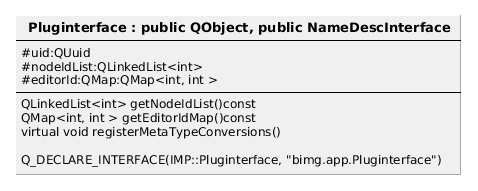
\includegraphics[width=1\textwidth]{pluginterface_diag.png}
  \caption{A pluginterface osztálydiagramja }

  \label{fig:bimg_slot_diag}
\end{figure}
\end{center}
Első lépésként definiáltam egy plugin interface osztályt, amely a Pluginterface nevet kapta. Azon túl, hogy a Q\_DECLARE\_INTERFACE() makró segítséggel egy interfészt deklarálása történik benne még három fő funkcionalitást különíthetünk el benne.
			\begin{itemize}
			\itemsep0em
			\item Tartalmaz egy UUID\cite{website:uuid_site} adattagot. Amely egy 128 bites állandó és egyedi azonosítója a pluginnak. A jelenlegi architektúrában ez a változó nem használt, azonban a további fejlesztési lehetőségek részben található PluginContainer és PluginUpdater rendszerek megkövetelik használatát. Ugyan ez érvényes a NameDescInterface által biztosított adattagokra is.
			\item Adott két előkészített tároló nodeIdList, és editorIdMap ahol különböző metatype-idk tárolására van lehetőség. (Konkrétan a Data-, Process- és IndicatorNodekhoz továbbá a SlotWidgetBasePartokhoz tartozó metatype-idkre.)
			\item Egy előkészített függvény: registerMetaTypeConversions(), amelyben definiálhatjuk a különböző saját fejlesztésű adattagok közötti konverziós lehetőségeket. 
		\end{itemize}

\subsubsection{Plugin metaobjektumok és ellenőrzések}
Ahogy fentebb említettem, több objektum metatípus leírója utazik a pluginnel. Gyakorlatilag ha valamelyik tárolóban eltárolunk metatype-id az betöltéskor beolvasásra kerül. Természetesen nem ellenőrzés nélkül, a minden plugin betöltéskor két szintű ellenőrzésen megy keresztül:
\begin{itemize}
	\itemsep0em
	\item A PluginLoader ellenőrzi, hogy egy szabványos pluginről van-e szó. Tehát Pluginterface ős osztállyal, és interfész deklarációval továbbá Q\_OBJECT makróval kell rendelkeznie (QObject osztályból örököltetni nem szükséges, hiszen a Pluginterface eleve a QObject osztály gyerekosztálya.) amint ez sikerrel lezárul a PluginLoader osztály létrehoz egy QPluginLoader pointert, amelyet a pluginLoaded signállal megküld a NodeManager osztálynak.
	\item A második szintű ellenőrzést a NodeManager::handlePluginLoaded(...) végzi. Végig iterál a beregisztrált azonosítókon. Tárolási helytől függően, vagy BaseNode, vagy SlotWidgetBasePart objektumot próbál készíteni a metatype rendszer segítségével. Amennyiben ezek valóban megfelelő típusú objektumoknak bizonyulnak beregisztrálja a saját tárolójába. A metatype-id konverziós definíciók regisztrálása is itt történik.
\end{itemize}

\subsubsection{NodeManager}
\begin{center}
\begin{figure}[h]
  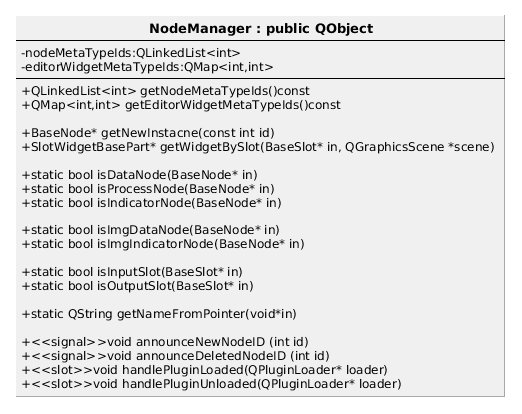
\includegraphics[width=1\textwidth]{nodeman_diag.png}
  \caption{A nodemanager osztálydiagramja }

  \label{fig:bimg_node_man}
\end{figure}
\end{center}
A NodeManager eléggé fontos architekturális szerepet tölt be a BIMG rendszerben. Ez az osztály tekinthető a pluginek és a BIMG közötti határvonalnak. Itt történik (a korábban már részletezett módon) a pluginok tartalmának beolvasása és ellenőrzése. Továbbá itt van lehetőségünk új példányokat igényelni ezekből az objektumokból, paraméterként átadott metatype-id segítségével. A NodeManager csak azokból az objektumokból készít új példányt, amelyek regisztrálva vannak nála. Ennek előnye, hogy ilyen módon letilthatóvá válnak bizonyos pluginek vagy plugin részek használata.

Például a későbbiekben tárgyalt NodePalette, először kikéri a regisztrált és érvényes metatype-idk listáját (getNodeMetaTypeIds()), majd a getNewInstacne(...) segítségével kér új példányokat az adott típusú objektumból.


\subsubsection{Egy példa plugin}
A plugin rendszer bemutatátás egy példával zárnám, ahol egy plugin létrehozásának menetét ismertetem:
\begin{enumerate}
\itemsep0em
\item Hozzunk létre egy szabványos C++ dinamikus függvénykönyvtárat, majd származtassuk le a Pluginterface ősosztályból, végül alkalmazzuk rajta a Qt-s interfész makrókat.
\begin{lstlisting}
//plugin_alpha.h
class PLUGIN_ALPHASHARED_EXPORT plugin_alpha : public Pluginterface
{
    Q_OBJECT
    Q_PLUGIN_METADATA(IID "org.examples.MyInterface")
    Q_INTERFACES(IMP::Pluginterface)

    //...
};
\end{lstlisting}
\item Készítsük el a saját nodejainkat, és adattípus konverzióinkat. Nodek esetén használjuk ősosztálynak valamelyik node típust (DataNode, ProcessNode vagy IndicatorNode). A típus konverzióknak a forrás objektum típusból egy const referenciát kell átvennie, és egy cél objektumot kell visszaadnia.
\begin{lstlisting}
//mat2image.h
Q_DECLARE_METATYPE(cv::Mat)
class Mat2Image{
public:
    static cv::Mat castImgToMat(const QImage& image);
    static QImage castMatToImg(const cv::Mat& mat);
\end{lstlisting}
A fenti kódban az OpenCV Mat objektum típuskonverziója történik meg QImage típusra és vissza. Megjegyzés: bármilyen külsős libbel végezzük a képfeldolgozást ajánlott a felhasznált adatformátumot ilyen módon regisztrálni.

\item A plugin konstruktorában regisztráljuk a metatípusokat! Illetve definiáljuk felül a registerMetaTypeConversions függvényt.
\begin{lstlisting}
//plugin_alpha.cpp
Q_DECLARE_METATYPE(RGBASplitter)
Q_DECLARE_METATYPE(RGBAJoin)

plugin_alpha::plugin_alpha():
    Pluginterface(QUuid::createUuid(),"PLUGIN_ALPHA","CORE FEATURES")
{
    //data
    this->nodeIdList<<qRegisterMetaType<DoubleDataNode>();
    this->nodeIdList<<qRegisterMetaType<StringDataNode>();
    //..
}
void plugin_alpha::registerMetaTypeConversions(){
    QMetaType::registerConverter<cv::Mat,QImage>(Mat2Image::castMatToImg);
    QMetaType::registerConverter<QImage,cv::Mat>(Mat2Image::castImgToMat);
}

\end{lstlisting}
\end{enumerate}


\subsection{InputList}
Az InputList az egyik legvékonyabb architekturális elem a BIMGben. Feladata roppantul egyszerű: lehetőséget ad a felhasználó számára, hogy összeállítson egy bemeneti listát, amelynek elemeit átadhatja a ProcessChain számára feldolgozásra. Lehetőségünk van egyszerre egy, vagy több elemet a listához hozzáadni, vagy eltávolítani. Továbbá előnézeti lehetőséget biztosít a felhasználó számára, aki így feldolgozásra küldés előtt megvizsgálhatja a nyers képet. Architekturális szempontból a currentPicSelectionChanged (QString) signaljának van a legnagyobb jelentősége, amely a ProcessChain számára küldi meg az éppen aktuális bemenet elérését.

\subsubsection{Input műveletek}
\begin{center}
\begin{figure}[h]
  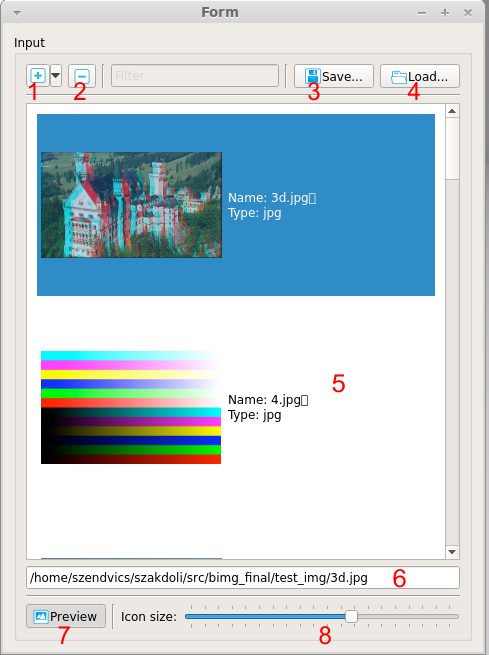
\includegraphics[width=0.5\textwidth]{user/fileeditor.png}
  \caption{Input műveleti ablakban elérhető lehetőségek.  }
1: Egy vagy több kép hozzáadása az input listához.\\2: Aktuális kép törlése az input listáról.\\3: Aktuális inputlista mentése.\\4: Korábban mentett inputlista betöltése.\\5: Aktuális input lista vizsgálati helye.\\6: Inputok gyors előnézeti területe.\\7: Gyors előnézeti mód ki/be kapcsolása.\\8: Gyors előnézeti mód méretének változtatása
  \label{fig:bimg_filelistdialog}
\end{figure}
\end{center}

\subsection{GUI}
Az eddig tárgyalt modulok, és alrendszerek (az InputList kivételével) nem rendelkeztek se grafikus, se más fajta felhasználói felülettel. Ezeknek a moduloknak a megfelelő interfészei használatával készítettem a grafikus felhasználói felületet. A GUI munkálatok kettő fontos részből álltak, az első részben a Qt által biztosított osztályokat bővítettem ki a projekt szempontjából szükséges funkcionalitásokkal. A másodikban ezekre támaszkodva készítettem saját fejlesztésű GUI elemeket, hiszen nem volt megfelelő gyári GUI elem ami képes lett volna megjeleníteni a DataNode, ProcessNode vagy IndicatorNode objektumokat.
\subsubsection{Scene\&View - guiview lib}
Architekturális szempontból a GUI peremén (a userhez a legközelebb), helyezkednek el a QGraphicsView és QGraphicsSenere gyermekosztályai.

\begin{center}
\begin{figure}[h]
  
\includegraphics[width=1\textwidth]{toolbar.png}
  \caption{A Base view toolbarja. (1: Nagyítás, 2: Kicsinyítés, 3: Méretezés értékhez, 4: Méretezés értékhez, 5. Forgatás jobbra, 6. Forgatás balra, 7: Forgatás adott értékhez, 8: Forgatás adott értékhez, 9: Interakciós mód, 10: Nézeti ablak beállításainak nullázása, 11: AAA engedélyezése/tiltása, 12: Simított bitkép transzformációk tiltása/engedélyezése , 13: OpenGL renderelés engedélyezése/tiltása, 14: Nézeti ablak jelenlegi tartalmának mentése) }
  \label{fig:bimg_viewgui_toolbar}
\end{figure}
\end{center}
A BaseView osztály egy Toolbar osztállyal párhuzamosan fejlesztve készült el. Segítségükkel a felhasználó alap interakciókra képes: zoomolni, forgatni a megjelenített grafikát a képen, adott objektumokat kijelölni és mozgatni, különböző renderelési opciókat ki és be kapcsolni, és az éppen aktuális megjelenítési állapotokról készült képet elmenteni. A BaseScene kapja el a Drag\&Drop és egyéb eseményeket, erre az osztályra építve készült el a NodeEditorScene. (További részletek a \ref{fig:bimg_viewgui}. ábráról olvashatóak le.)
Ezeknek a kis osztályoknak a tervezésénél és implementációjánál kifejezetten arra törekedtem, hogy ne kerüljön ide a BIMGhez köthető funkcionalitás, adattag stb, így jelenleg egy külön statikus libként van a BIMGbe bele forgatva guiview néven.
\begin{center}
\begin{figure}[h]
  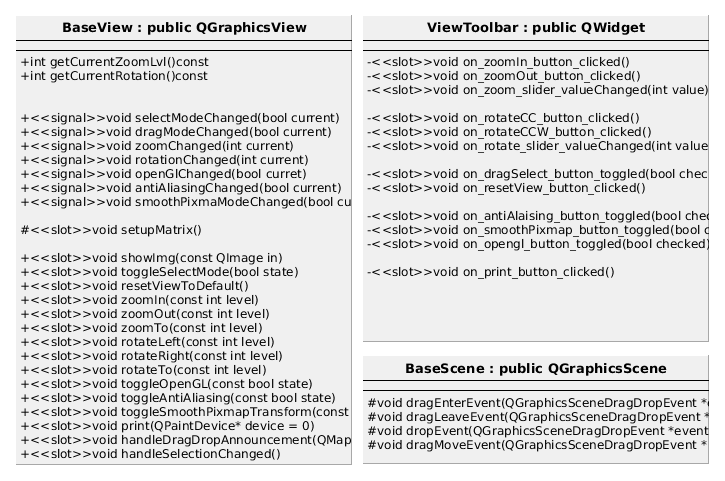
\includegraphics[width=1\textwidth]{viewgui_dia.png}
  \caption{A ViewGui libnek az osztálydiagramja}
  \label{fig:bimg_viewgui}
\end{figure}
\end{center}

\subsubsection{NodePalette/NodePaletteForm}
A NodePalette biztosítja a felhasználó számára, hogy a BIMG rendszerben található nodekat használhassa, illetve bővebb információt szerezhessen róluk. A nodek a könnyebb rendszerezhetőség érdekében füleken jelennek meg. A csoportosítás alapja a BaseNode::category (QString) változónak a tartalma, amelyet az adott node konstruktorában adhat meg a fejlesztő. (Ugyan ezen a módon definiálható a node, neve, leírása, súgó szövege és mini-iconja.) A Nodehoz tartozó súgás jelenleg egy jobb kattintással hozható elő. Az új node létrehozása rendkívül egyszerű: hiszen elég az NodePalettán található elemet a közismert fogd és vidd módszerrel a NodeEditor felületére mozgatni. (\ref{fig:bimg_nodepalette}. ábra)
\begin{center}
\begin{figure}[h]
  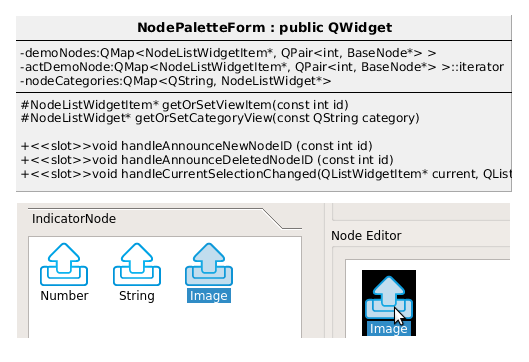
\includegraphics[width=1\textwidth]{nodepalette.png}
  \caption{A NodePalette osztálydiagramja, és működés közbeni fotója }
  \label{fig:bimg_nodepalette}
\end{figure}
\end{center}

Architekturális szempontból a NodePalette (NodePaletteForm), gyakorlatilag a NodeManager részére képez egy viewet. Követlen értesítést kap (announceNewNodeID (int id), announceDeletedNodeID (int id) signáljai a NodeMangernek) a frissen regisztrált, és az éppen letiltott metatype-idkről. A handleAnnounceNewNodeID(int) és handleAnnounceDeletedNodeID(int) slotokkal kezeli ezeket az értesítéseket. Minden egyes metatype-idhez kér a palette egy demo node példányt a managertől. Ezek a nodek, csak arra szolgálnak, hogy a NodePalette információt tudjon szolgáltatni a felhasználó részére a noderől. (Tehát feldolgozási sorhoz nem lesznek hozzáadva stb.)

\subsubsection{NodeEditor/NodeEditorScene}
A megjelenítési műveletek eseménykezelő és elem mappoló színhelye. A ViewGUI::BaseScene osztálynak a gyermekosztálya. Fogadja a drag\&drop illetve egyéb más felhasználói interakciókat, minimális logikával rendelkezik: gyakorlatilag megszűri az eseményeket. Minden lehetséges BIMG szempontból érdekes eseményt továbbít a ProcessChainView, részére. pl.: Ha elkap egy drop műveletet, akkor ellenőrzi, hogy az adott objektum MIME típusa érdekes lehet-e a BIMG számára.
Jelenleg ilyen figyelt metatípusok a: "application/x-qabstractitemmodeldatalist" ha tartalmaz Node metatype-idt (ez a Qt::UserRole+2048-as role), a "application/x-bimgnodeconnector", amely akkor érvényes, ha tartalmaz "sourceobj" Stringgel indexel adatot. Az első mimeadat a NodePaletteről történő fogd és vidd művelet eredménye a második két NodeWidgetSlotConnection közötti kapcsolat létrehozási kísérlet eredménye.

\subsubsection{ProcessChainView}
Ha a Node-Slot-Parameter rendszer feldolgozó logikája a ProcessChain volt akkor várható, hogy a ProcessChainView is hasonló architekturális feladatokat tölt be (csak a view oldalon).
Ez az állítás helytálló. A következő listában röviden összegzem a feladatokat, a lentebb található osztálydiagramon pedig megtalálhatóak ezek a feladatokhoz megfeleltethető függvények és adattagok.
\begin{itemize}
	\itemsep0em
	\item Itt tárolódik és konfigurálódik a NodeWidgeteket. (pl: itt kerül beállításra a NodeEditorScene elérése stb.)
	\item Fogadásra és feldolgozásra kerülnek a NodeWidgetek különböző kérelmeit: klónozás, és törlés.
	\item Fogadásra kerül a NodeEditorScenetől érkezett és előfeldolgozott eseményeket. Az események-NodeWidgetek kimappolása és ellenőrzése is itt történik pl. 2 Slot összekapcsolási kérelme esetén
	\item Itt történik az információ csere a ProcessChainnel, a feldolgozás jelenlegi állapotáról, továbbá az új és törölt (illetve hozzáadni és törölni kívánt) nodekről.
\end{itemize}

\begin{center}
\begin{figure}[h]
  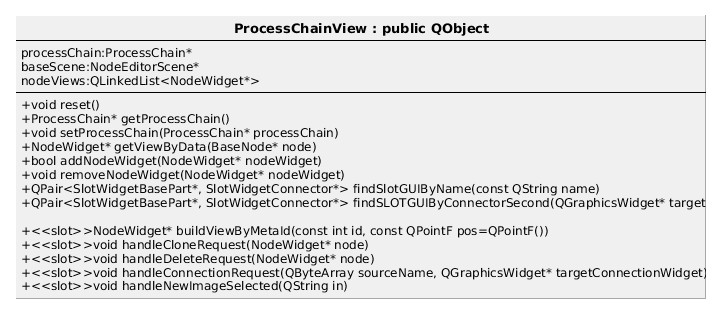
\includegraphics[width=1\textwidth]{processcahinview.png}
  \caption{A ProcessChainView osztálydiagramja}

  \label{fig:bimg_processchainview}
\end{figure}
\end{center}

\subsubsection{NodeWidget}
A GUI fejlesztésben a NodeWidget alrendszer tervezése és implementálása jelentette a legnagyobb kihívást. A NodeWidget a QGraphicsWidget osztályra lett felépítve. A widget több rész widgetre bontható fel:
\begin{itemize}
	\itemsep0em
	\item NodeWidgetBasePartokra amelyek közvetlenül a BaseNode valamely elemét jelenítik meg
	\item SlotWidgetBasePartokra amelyek közvetlenül egy darab slot megjelenítését és kezelését végzik
\end{itemize}
A NodeWidget azontúl, hogy levezényli a hozzárendelt BaseNode megjelenítését (az alap adatok vizualizálásán túl, az esetleges slotok megjelenítését és kezelését). Különböző kéréseket is küldhet a ProcessChainViewnek. Jelen implementáció alapján kettő kérés érkezhet egy NodeWidgettől: az egyik a clone, azaz hogy egy vele azonos típusú NodeWidget kerüljön fel a megjelenítőre (és Node letárolásra a ProcessChainben); a másik a delete, azaz törlés tehát amikor a NodeWidget saját maga eltávolítását kérvényezi a ProcessChainViewből és ProcessChainból.

A NodeWidget tartalmának elrendezése és kirajzolása egy GridLayout segítségével került megvalósításra.
\begin{center}
\begin{figure}[h]
  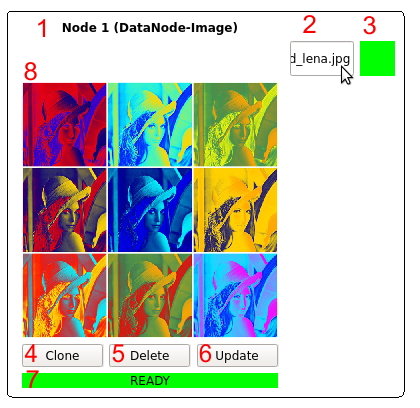
\includegraphics[width=0.7\textwidth]{datanode_full.png}
  \caption{Egy image DataNode. (1: A Node neve. 2: A DataNode output slot szerkesztésének helye (jobb klikkel további funkciók érhetőek el.). 3. Node isReady staus indicator. 4. Klónozás 5. Törlés. 6. Frissítés 7. Node státusz állapota. 8. Kisméretű előnézeti kép.)}
  \label{fig:datanode_full}
\end{figure}
\end{center}
Ezen az ábrán (\ref{fig:datanode_full}.) egy Image típusú DataNodet láthatunk. Jelen példa esetben a rendszer nem az InputList által átadott képet tartalmazza magában, hanem egy a felhasználó által kiválasztottat. Továbbá látható, hogy a node isReady státusza true tehát azonnal végrehajtható (ez az alsó READY feliratból olvasható ki), és hogy az egy datab outputslotja is készen áll a végrehajtásra. Az input slotok mindig a node bal oldalán foglalnak helyet, még az output slotok a node jobb oldalán. Jelen esetben mint a 3 alapvető funkció gomb elérhető, a clone, delete és update is.

\subsubsection{NodeWidgetBasePart}
Egy-egy alap NodeWidget elem megjelenítését, és kezelését egy-egy NodeWidgetBasePart végzi. Osztálydiagramja lentebb látható. Két fontos adattagja van: first és second. Ahogy a diagramon látható a first egy QWidget még a second egy QGraphicsWidget. NodeWidgetBasePart legfontosabb feladata, hogy eltároljon egy widgetet (ez lehet akár saját készítésű widget is). Majd az initFirst() függvénnyel inicializálja first nevű widgetet (feltölti a BaseNodeból származó adatokkal), a művelet végén a first widgetet, pedig adja hozzá a scene pointer által mutatott QGraphicsScenehez. A GraphicsScenehez történő hozzáadás egy proxy osztályt ad vissza, amelynek memóriacímét letárolja a second pointerrel. A proxy osztály lehetőséget biztosít, hogy szokásos QWidget osztályt, megjeleníthessünk a QGraphicsViewen. 
A NodeWidgetBasePart a külvilág felé egy slotot biztosít: ez az update(), mellyel szinkronizálhatóak a BaseNode és a first widget közötti adatok. 
Példákat NodeWidgetBasePart osztályokra: a \ref{table:nodewidgetparts} táblázatban találhatunk.
\begin{table}[h]
%\begin{tabular}{@{}rl@{}}
\begin{tabular}{p{5.5cm}|p{7.5cm}}

\toprule
\multicolumn{1}{c}{\textbf{Név}} & \multicolumn{1}{c}{\textbf{Feladat és eszköz}} \\ \midrule
\textbf{NodeWidgetTitle} & Megjeleníti az aktuális BaseNode címét (Ez a cím a BaseNode nevéből kategóriájából és a ProcessViewen betöltött sorszámából adódik). (QLabel)\\
\hline
\textbf{NodeWidgetPreviewPixmap} & Előnézeti pixmap, DataNodek esetén a bemeneti kép jelenik meg itt, IndicatorNodek esetén az éppen kiszámolt kimeneti kép. (QPixmap és QLabel) \\
\hline
\textbf{NodeWidgetStatusLab} & A node isReady státusza jelenik meg itt. (QLabel) \\
\hline
\textbf{NodeWidgetCloneButton} & Egy nyomógomb aminek segítségével kérvényezheti a NodeWidget a ProcessChainView felé a klónozást. (QPushButton) \\
\hline
\textbf{NodeWidgetDeleteButton} & Egy nyomógomb aminek segítségével kérvényezheti a NodeWidget a ProcessChainView felé a saját maga eltávolítását. (QPushButton) \\
\hline
\textbf{NodeWidgetBaseUpdateButton} & Frissítés indul fut le a NodeWidgeten. (A felhasználó saját maga kezdeményezheti a NodeWidget manuális frissítését \\ 
\hline

\end{tabular}
\caption{A NodeWidget részei}
\label{table:nodewidgetparts}
\end{table}

\begin{center}
\begin{figure}[h]
  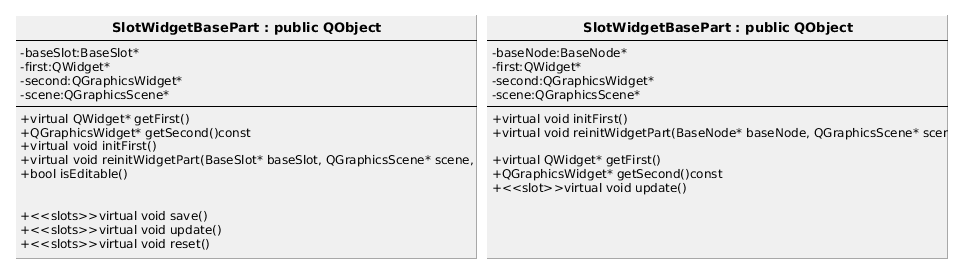
\includegraphics[width=1.1\textwidth]{node_slot_widgetpart.png}
  \caption{A NodeWidgetBasePart és a SlotWidgetBasePart osztályok diagramja}

  \label{fig:bimg_widget_slot_view_diag}
\end{figure}
\end{center}

\subsubsection{SlotWidgetBasePart}
A SlotWidgetBasePart osztály működését tekintve nagyon hasonló a NodeWidgetBaseParthoz. A különbség annyi, hogy ebben az esetben egy slot megjelenítéséről gondoskodunk. Továbbá bizonyos esetekben van lehetőségünk, hogy a slot által hordozott paramétert szerkeszthetővé tesszük. Ezt DataNodek outputslotjai esetén tehetjük meg. Erre azért van szükség, hogy a ProcessChainbe más adat is kerülhessen ne csak az InputListről kapott kép. (pl.: konstans) Mivel új adattípusok is érkezhetnek a pluginekkel ezért a pluginekbe ilyen SlotWidgetBasePart osztályokat is csomagolhatunk. (Ahogy azt a Plugin rendszer bemutatása során leírtam.)

A SlotWidgetBasePart kezelése egyszerű: a biztosított editor felületen szerkeszthetjük az adatot: pl.: szám esetén ez egy számbeviteli mező lesz, ahova bevihetjük a kért számot. Amint az editor elveszíti a fókuszt a benne lévő adat mentésre kerül. Azonban ha biztosra szeretnénk menni jobb kattintással az editorban kiválaszthatjuk a kívánt funkciókat.
2 slotot úgy tudunk összekötni, hogy a kis slot állapotot jelző indikátor mezőt megfogjuk és fogd és vidd módszerrel egy másik slot indikátor mező fölött elengedjük. Ha jó slot összekötését kezdeményeztük, akkor a kapcsolat automatikusan létrejön a két node között.

\begin{center}
\begin{figure}[h]
  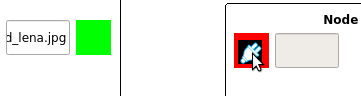
\includegraphics[width=0.7\textwidth]{connection.png}
  \caption{Slotok összekapcsolása}

  \label{fig:bimg_just connection}
\end{figure}
\end{center}
Két slot közötti kapcsolat létrehozatalának pillanata. Fontos megjegyzés: Látható, hogy az output slot zöld tehát készen áll a végrehajtásra, még az inputslot piros tehát még nem érkezett rá adat.


\section{A Fejlesztés részletei}
\subsection{Fejlesztési napló}
A fejlesztés során iteratív fejlesztési módot követtem. Az alapvető jellemző metodikám az volt, hogy kiválasztottam egy modult, aminek a legfontosabb funkcióit vázlatosan megterveztem. Ha az adott modul első iterációjáról volt szó akkor egy külön teszt projektben készítettem el az első verziót. (Így lehetőségem, volt az új funkciókat úgy tesztelni esetlegesen újra tervezni átvariálni, hogy közben a rendszer többi részével nem kellett hosszas munkaórákat töltenem, hogy képes legyen együttműködni az esetlegesen később teljesen megváltoztatott architektúrával.) Az fejlesztés során összegyűlt tapasztalatokat bugokat, esetleges új funkció kéréseket mindig a következő iterációban vettem csak figyelembe. Egy iteráció hossza 1-3 nap volt. A következő felsorolásban vázolom, hogy melyik modulok, alrendszerek fejlesztése tartozott egy iterációba.
\subsubsection{Iterációk}

\begin{enumerate}
\itemsep0em
\item Node-Slot-Parameter rendszer kezdetei tervei és Proof of Concept implementációja. (template)
\item Input modul megtervezése és implementálása, Viewgui és settings libek elkészítése.
\item Node-Slot-Parameter rendszer teljes revíziója és újratervezése. (metatype), Qt Pluginrendszerének vizsgálata, és állatorvosi lovának elkészítése, a későbbi tervezés megkönnyítéséhez.
\item ProcessChain tervezése és implementálása (körkereséssel és gráfelemzéssel), Node-Slot-Parameter rendszer tesztei és javítása, saját metatípussal rendelkező slotok tesztje.
\item OpenCV - Qt wrapper megtervezése, implementálása és tesztje
\item OpenCV - Qt wrapper revíziója
\item Pluginrendszer megtervezése és első plugin elkészítése
\item Teljes refaktor: Első mérföldkő működőképes Node-Slot-Parameter rendszer és Plugin rendszer, (OpenCV-Qt konverziók még mindig nem 100\%osak)
\item ProcessChain áttervezése és implemetálása
\item NodePalette elkészítése és NodeEditor első verziója
\item NodeEditor áttervezése és implementálása
\item NodePartWidgetek és SlotPartWidgetek megtervezése és implementálása
\item BaseScene és ProcessChainView szétválasztása
\item Második mérföldkő: kezdetleges GUI működik
\item GUI csiszolása, tesztek, bugfixek
\item Bugfix + alpha plugin fejlesztése
\item Deploy rendszerek előkészítése (dupla hosszúságú lett végül)
\item Bugfix, elmaradt apró funkciók pótlása
\item Deploy + Dokumentáció bővítése és korrigálása (papír alapú dokumentációk digitalizálása)

\end{enumerate}

\subsubsection{Névterek és libek}
A legfontosabb modulokat, alrendszereket a könnyebb rendszerezés, és az egyszerűbb kód-újrafelhasználás miatt külön lib-be és névterekbe csomagoltam. A következő két táblázat ezeket mutatja be a legfontosabb szervező logikákkal együtt. \\ A namespaceket a \ref{table:bimg_namespace} táblázat tartalmazza. A libeket a \ref{table:bimg_libs} táblázat tartalmazza. 
\begin{table}[h]
%\begin{tabular}{@{}rl@{}}
\begin{tabular}{p{1cm}|p{12cm}}

\toprule
\multicolumn{1}{c|}{\textbf{Névtér}} & \multicolumn{1}{|c}{\textbf{Leírás}} \\ \midrule
\multicolumn{1}{c|}{\textbf{IMP}}  & Itt található minden, alapvető osztály, amelyek szorosan kapcsolódnak a Node-Slot-Parameter rendszerhez. Ebbe a névtérbe kerülnek a be a pluginekben fejlesztett Nodek is.\\
\hline
\multicolumn{1}{c|}{\textbf{VIEWGUI}}  &  A legalapvetőbb megjelenítési funkciókat magukba záró osztályok lelőhelye.\\
\hline
\multicolumn{1}{c|}{\textbf{BIMG}}  & A BIMG rendszer fő névtere, itt található minden amit az IMP felett van architekturálisan: Plugin és Input kezelés, ProcessChain, NodePalette stb. \\
\hline

\end{tabular}
\caption{A BIMG rendszerben található névterek és szerveződésüknek legfontosabb logikája }
\label{table:bimg_namespace}
\end{table}


\begin{table}[h]
%\begin{tabular}{@{}rl@{}}
\begin{tabular}{p{1cm}|p{12cm}}

\toprule
\multicolumn{1}{c|}{\textbf{Név}} & \multicolumn{1}{|c}{\textbf{Funkció}} \\ \midrule
\multicolumn{1}{c|}{\textbf{bimg\_imp}}  & Gyakorlatilag a teljes Node-Slot-Paramter rendszer és a minden szükséges architekturális és GUI elem alapját képező osztály megtalálható itt, ami ahhoz szükséges egy saját plugin fejlesztéséhez. (statikus linkelésű)\\
\hline
\multicolumn{1}{c|}{\textbf{guiview}}  &  Alapvető grafikus megjelenítők lelőhelye a QGraphicsScene és a QGraphicsView felett található osztályok, amelyek önállóan is hasznosíthatóak bármely GUI-s alkalmazáshoz. (statikus linkelésű)\\
\hline
\multicolumn{1}{c|}{\textbf{settings\_lib}}  & QSettings felett működő minilib. (Jelenleg még inkább snippset.) (statikus linkelésű)\\
\hline
\multicolumn{1}{c|}{\textbf{plugin\_alpha}}  & A BIMG magját képező nodek, feldolgozó egységet és a Qt-OpenCV konverziós megfeleltetések lelőhelye. (dinamikus linkelésű plugin)\\
\hline
\multicolumn{1}{c|}{\textbf{qslog\_lib}}  & Egy nagy kompakt Qt-s loggerlib\cite{website:qslog_site} amelyet razvanpetru publikált bsd licence alatt. (statikus linkelésű)\\
\hline

\end{tabular}
\caption{A BIMG rendszert felépítő libek listája }
\label{table:bimg_libs}
\end{table}
\subsubsection{Nehézségek}
A projekt tervezése, implementálás során több nehézség is adódott. Az egyik jelentősebb a Node-Slot-Parameter rendszer kidolgozása körül volt a Slotok kapcsolatainak kezelése kapcsán. (Hogyan és mikor legyenek lebontva a kapcsolatok, hogy ne fordulhasson elő inkonzisztens állapot. A másik probléma a tárol adatok konverziójával volt, hogy milyen módon lehetséges egy tetszőleges új saját típusra konvertáló függvényt regisztrálni a metatype rendszerbe. Mind a kettő problémát sikeresen megoldottam és a dolgozat korábbi fejezeteiben mindegyiket bemutattam.

A pluginrendszer sok gondolkodást és tervezést okozott, hogy hogyan lehet elegánsra és biztonságosra megtervezni, hogy egy hibásan megírt node, vagy plugin ne okozzon túl nagy problémát. Erre csak részleges megoldás született: a rendszer minden kivételt elkap és megpróbálja feldolgozni (egy hibaüzenettel megállítja a feldolgozást és közli, hogy honnan érkezett a hiba). Azonban ez csak az hibaesetek egy részére hozott megoldást pl.: ha a nodeban szegmentálásihiba történik, akkor azt ilyen módon nem lehetséges jól kezelni. A megoldásra terveket már készítettem, azonban a jelenlegi architektúra jelentős szintű utólagos megváltoztatását igényelte volna. Amire jelenelg sajnos nem volt lehetőségem. A terv lényege annyi, hogy a egy PluginContainer szolgáltatást hozunk létre a háttérben, amelyre a BIMG valamilyen módon felcsatlakozik, megadja a végre hajtani kívánt Node metatype-idjét és a bemeneti és kimeneti slotok adattípusát és jelenlegi állapotát, a service elvégzi a számításokat, majd visszatér az eredményekkel. A service mindig tárolja a legutolsó kérést ezért ha pl szegmentálási hiba keletkezik akkor képes az adott node tiltására. Amennyiben a pluginContainer adott időszakon belül nem küld választ a BIMG részére akkor a BIMG megállíthatja és újraindíthatja azt.

\subsubsection{Tesztek}
A fejlesztés során a különböző rendszerek, alrendszerek, modulok, osztályok és függvények folyamatosan tesztelve voltak. Ezek a tesztek jó része kézzel történt. Készült pár félautomata teszt eset is (ezek elsősorban a Node-Slot-Parameter rendszerhez készültek.

Alább látható egy teszteset kimenetele:
\begin{lstlisting}
Starting /home/szendvics/szakdoli/src/bimg5/bimg/build-bimg_imp-Desktop_Qt_5_2_1_GCC_32bit_595617-Debug/bimg_imp...
############################################
#Base Node system test
############################################
DefaultData       1
DefaultIndicator  0
NewValue          11
TargetResult      22
############################################
"#Init:                " PASSED!
"#Connectors:          " PASSED!
"#Setter&Conv:         " PASSED!
"#Getter&Conv:         " PASSED!
"#EXEC-DATA:           " PASSED!
"#EXEC-CONTROL:        " PASSED!
"#EXEC-VIEW:           " PASSED!
"#ISREADY FULL RESULT: " PASSED!
"#After Exec DataCheck:" PASSED!
GENERAL STATE          : true   9 / 9
############################################
\end{lstlisting}
Ebben a tesztesetben a korai fejlesztésú Node-Slot-Parameter rendszert teszteltem. Konkrétan két slot közötti információáramlás helyességét azonos és különböző (de konvertálható adattípusok esetén). Egy teszt több kisebb tesztesetből áll. Először a teszt fejléce kerül megjelenítésre: a teszt neve és használt bemeneti paraméterek és a várt kimeneti paraméterek. Utána következnek a tesztesetek eredményei, majd egy összegzés, hogy hányból hány teszt sikerült. 

\subsection{Az elkészült munka értékelése}

Munkám során megterveztem és kifejlesztettem egy képfeldolgozást támogató keretrendszert, amely alkalmas képek egyedi vizsgálatára és kötegelt feldolgozására. A rendszer képes különböző (fájl)formátumokban és módokon vizualizálni az eredményképeket. A paraméterezhető képfeldolgozási algoritmusokat dinamikusan betöltődő modulok biztosítják, és egy egyszerű (bár jelenleg még nem túl kompakt) könnyen kezelhető grafikus felületen lehetőség van többlépcsős feldolgozás megvalósítására is. A rendszer ingyenes modern és nyíltforráskódú technológiák felhasználására épült.

A program még kűzd kisebb hibákkal, hiányosságokkal, gyermekbetegségekkel azonban az alap feladatai ellátásra alkalmas.

\subsection{További fejlesztési lehetőségek}
A következő pár pontban röviden bemutatom, hogy az adott modulok milyen további fejlesztési lehetőségeket foglalnak magukban.
\subsubsection{Plugin rendszer}
Egy bizonyos plugin szám felett elkerülhetetlen lesz a pluginek teljes körű managelése. Ide értem, az aláírással és egyedi azonosítóval történő azonosításukat. Ennek legegyszerűbb oka az, hogy jól karban tartott pluginrendszernél is előfordulhatnak hibák, ilyenkor az adott plugint frissíteni kell. Erre célszerű egy automatikus frissítési modult elkészíteni. További ötletként felmerült egy központi plugin repository lehetősége is a jövőben, ahol a felhasználó szabadon összeválogathatja a számára szükséges plugineket.
\subsubsection{GUI}
A NodeWidgetek kompaktabbá tétele sokat segíthetne, a nagyobb feldolgozási láncok megalkotása során. (több nodet lehet látni egyszerűbb a komplexebb ProcessChainek kialakítása)
\subsubsection{Optimalizálási lehetőségek}
\begin{itemize}
	\itemsep0em
	\item A ProcessChain feldolgozás párhuzamosítása.
	\item  A FileInput kezelő bélyegképes előnézeti funkciójának több szálúsítása.
\end{itemize}


\subsection{Használati útmutató}
Mivel korábban részletesen bemutattam a szoftver terveit, fejlesztését és működését, itt csak a legfontosabb hivatkozásokat gyűjtöm össze.
\begin{itemize}
	\itemsep0em
	\item \textbf{Input kezelés:}  InputList
	\item \textbf{Node Palette használata:}  NodePalette/NodePaletteForm
	\item \textbf{Node Editor használata:} ProcessChain, Scene\&View - guiview lib, NodeWidget, NodeWidgetBasePart, SlotWidgetBasePart
\end{itemize}

\subsection{Fejlesztői útmutató}
A BIMG vagy valamely plugin fejlesztéséhez elsődlegesen ez a dolgozat szolgál információforrásul. A forráskódok Doxygenes kommenteléssel készültek ezért, abból generálható részletes dokumentáció. Egy előkészített DoxyGen konfigurációs fájl és egy legenerált teljes dokumentáció is megtalálható a mellékletben. A forráskódok könyvtárában: \emph{Doxyfile} néven.
\subsection{Telepítési útmutató}
A BIMG esetében két féle telepítés mód járható.
\subsubsection{Forráskódból}
\begin{enumerate}
\itemsep0em
\item Ez esetben a program forráskódjára lesz szükség (amely a mellékletben megtalálható).
\item Telepített Qt 5.2.1es verzióra vagy újabbra.
\item Telepített 2.4.8as OpenCVre és forráskódjaira.
\item Nyissuk meg a bimg.pro fájlt QtCreatorban. Ellenőrizzük a subprojektekben a libeknek és includoknak az elérési útvonalát.
\item Fordítsuk le a szoftvert, és már használhatjuk is.
\end{enumerate}

\subsubsection{Binárisból}
A mellékleten több bináris deploy is megtalálható összezippelve. Elnevezésük a következő képpen alakul: bimg\_dátun\_deploy\_PLATFORM.zip
Cél paltformok:
\begin{itemize}
	\itemsep0em
	\item Linux Mint Maya (Qt 5.2.1, OpenCV 2.4.8 32bit)
	\item Windows 7 (Qt 5.2.1, OpenCV 2.4.8 64bit)
\end{itemize}
Amint megtaláltuk a számunkra megfelelő zip fájlt tömörítsük ki egy testszőleges könyvtárba. Más dolgunk nincsen az archívumban megtalálható az összes szükséges függvénykönyvtár és konfigurációs fájl, amely a BIMG futtatásához szükséges.

\begin{figure}[h]
  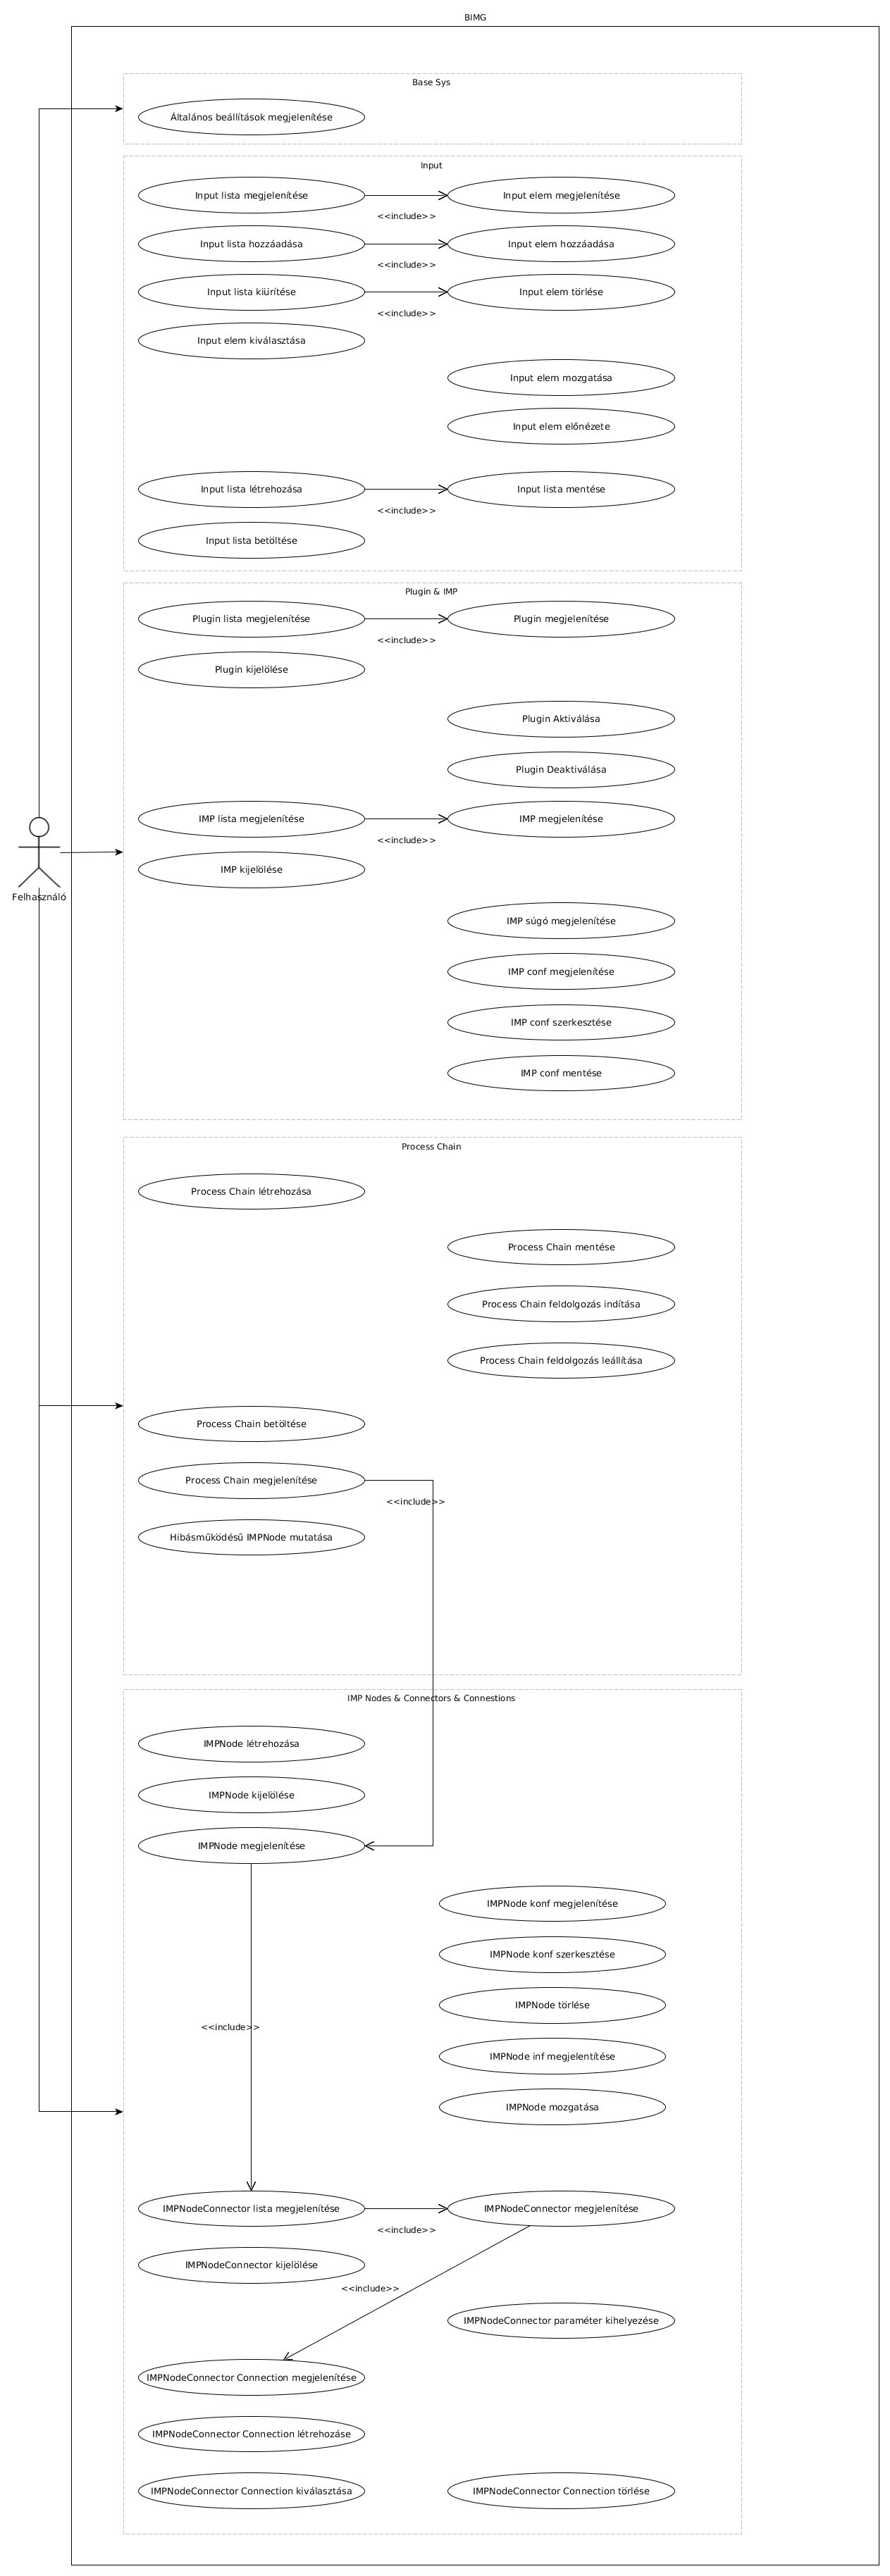
\includegraphics[width=1\textwidth]{usecase_full.png}
  \caption{A BIMG sematikus usecase diagramja }
  \label{fig:bimg_usecase_full}
\end{figure}


%\renewcommand{\bibname}{Irodalomjegyzék}
%\bibliographystyle{pemik}
%\bibliography{irodalomjegyzek}

\begin{thebibliography}{99}

    \bibitem{book:usecase_book_brief}
		Craig Larman (2004). 
        {\em Applying UML and Patterns, Prentice Hall, 3 edition 6.7 (66)(127)\\}

    \bibitem{book:pipelining_def}
		Jack J. Dongarra (1995). 
        {\em Numerical Linear Algebra on High-Performance Computers (3)\\}
        
 	\bibitem{website:valve_shading_tree}
		http://www.valvesoftware.com/publications/2006/\\SIGGRAPH06\_Course\_ShadingInValvesSourceEngine\_Slides.pdf
        {\em Valve, Jason Mitchell (2007), Shading in Valve’s Source Engine  (37) \\}     
        
        

    \bibitem{website:imagej}
        http://imagej.nih.gov/ij/
        {\em ImageJ - Image Process and Analysis in Java}
        
    \bibitem{article:imagej_article}
		Tony J. Collinsm,
        {\em ImageJ for microscopy}
        BioTechniques 43:S25-S30 (July 2007)

    \bibitem{website:imbatch}
        http://www.highmotionsoftware.com/products/imbatch\\
        {\em ImBatch - Batch Image Processing Software}

    \bibitem{website:originlab}
		http://www.originlab.com/index.aspx?go=Products/Origin/DataAnalysis/ImageProcessing\\
        {\em OriginLab - Image Processing}
        
        
    \bibitem{website:originlab_about}
        http://www.originlab.com/index.aspx?go=COMPANY/AboutUs\\
        {\em OriginLab - About Us}

    \bibitem{website:originlab_usd}
		http://www.originlab.hu/Originv9\_USD\_NEW\_20121022\_WEB.pdf\\
        {\em OriginLab - Licences}
        
	\bibitem{website:ibm_capture_req}
        http://www.ibm.com/developerworks/rational/library/4706.html\\
        {\em IBM - Capturing Architectural Requirements}  


	\bibitem{website:ni_blocks}
		http://zone.ni.com/reference/en-XX/help/371361J-01/lvconcepts/blockdiagram/\\
        {\em NI - LabVIEW 2012 Help - Block Diagram}  

	\bibitem{website:udk_blueprint}
		https://docs.unrealengine.com/latest/INT/Engine/Blueprints/Editor/index.html\\
        {\em UDK4 - Blueprint Editor Reference}  


	\bibitem{website:qt_about}
		http://qt.digia.com/About-Us/\\
        {\em QT - About } 
 
	\bibitem{website:qt_dochome}
        http://qt-project.org/doc/\\
        {\em QT - Doc} 
         
  	\bibitem{website:qt_docforum}
        http://qt-project.org/forums\\
        {\em QT - Forums}        

  	\bibitem{website:qt_docmaillist}
          http://lists.qt-project.org/mailman/listinfo \\
        {\em QT - MailingLists}        


	\bibitem{website:qt_in_use}
        http://qt.digia.com/Qt-in-Use/\\
        {\em QT Digia - In Use}  
        
        
	\bibitem{website:opencv_about}
        http://opencv.org/about.html\\
        {\em OpenCV - About}  
        
        
	\bibitem{website:qt_1_million}
		http://blog.qt.digia.com/blog/2014/04/16/qt-5-2-over-1-million-downloads/\\
        {\em QT Digia - Over 1 million}  
        
	\bibitem{website:soft_req_def}
        http://www.math.unipd.it/~tullio/IS-1/2007/Approfondimenti/SWEBOK.pdf\\
        {\em Guide to the Software Engineering Body of Knowledge, Chapter 2 - SOFTWARE R EQUIREMENTS}
        
        
	\bibitem{website:soft_func_req_ibm}
		http://www.ibm.com/developerworks/rational/library/4706.html\#N10098 \\
        {\em IBM - Capturing Architectural Requirements, Functional Requirements }
        
    \bibitem{publication:soft_nonfunc_req}
		Ruth Malan and Dana Bredemeyer
		http://www.bredemeyer.com/pdf\_files/NonFunctReq.PDF \\
        {\em Architecture Resources For Enterprise Advantage (2)\\}
        

	\bibitem{website:opencv_about}
        http://opencv.org/about.html\\
        {\em OpenCV - About}  

	\bibitem{website:qt_metatype_1}
		http://qt-project.org/doc/qt-5/qmetatype.html\#Q\_DECLARE\_METATYPE\\
        {\em Qt - Q\_DECLARE\_METATYPE}  

	\bibitem{website:qt_variant}
		http://qt-project.org/doc/qt-5/qvariant.html\#canConvert\\
        {\em Qt - QVariant konverziók}  

	\bibitem{website:qt_plugin}
		http://qt-project.org/doc/qt-5/plugins-howto.html\\
        {\em Qt - Plugins}  

	\bibitem{website:uuid_site}
		http://www.ietf.org/rfc/rfc4122.txt\\
        {\em Standards Track  - A UUID URN Namespace (RFC 4122) }  
        
	\bibitem{website:qslog_site}
		https://bitbucket.org/razvanpetru/qt-components/overview\\
        {\em QsLogger Lib }  

\end{thebibliography}


\section{Mellékletek}



\subsection{Felhasználói útmutató}

\subsection{CD melléklet}
A szakdolgozat CD mellékletének könyvtárszerkezete:

% itt a csel a [], amivel nem rak ki pontokat a latex
\begin{itemize}
    \item[] /VargaMarcell-DVLKHU-szakdolgozat.pdf
    \item[] /szakdolgozat-forraskod
    \begin{itemize}
        \item[] /diagramok
%        \item[] /kepek
%        \item[] /wireframek
        \item[] /szakdolgozat.tex
    \end{itemize}
    
    \item[] /rendszer-forraskod
    \begin{itemize}
 %       \item[] /app
        \item[] /src
        \begin{itemize}
  %          \item[] /google-api-php-client
            \item[] /Szakdolgozat
   %         \begin{itemize}
    %            \item[] FelhasznaloBundle
     %           \item[] JegyzokonyvBundle
      %          \item[] SzakdolgozatBundle
       %         \item[] UlesBundle
%            \end{itemize}
        \end{itemize}
        
%        \item[] /uploads
%        \item[] /web
    \end{itemize}
    
    \item[] /internetes-hivatkozasok

\end{itemize}

\end{document}